%%
%%
%% document.tex for doctorat
%%
%% Made by Philippe THIERRY
%% Login   <Philippe THIERRYreseau-libre.net>
%%
%% Started on  mar. 24 nov. 2009 19:46:57 CET Philippe THIERRY
%% Last update mer. 01 sept. 2010 21:30:18 CEST Philippe THIERRY
%%

%%%%%%%%%%%%%%%%%%%%%%%%%%%%%%%%%%%%%%%%%%%%%%%%%%%%%%%%%%%%%%%%%%%%%%%%%%%%%
%% Document style definition
%%%%%%%%%%%%%%%%%%%%%%%%%%%%%%%%%%%%%%%%%%%%%%%%%%%%%%%%%%%%%%%%%%%%%%%%%%%%%

\documentclass[twoside,a4paper,11pt,titlepage]{book} 	% document type


%%%%%%%%%%%%%%%%%%%%%%%%%%%%%%%%%%%%%%%%%%%%%%%%%%%%%%%%%%%%%%%%%%%%%%%%%%%%%
%% Packages integration
%%%%%%%%%%%%%%%%%%%%%%%%%%%%%%%%%%%%%%%%%%%%%%%%%%%%%%%%%%%%%%%%%%%%%%%%%%%%%

\usepackage[hundred]{vrsion}				% versioning support
\usepackage[latin1]{inputenc}				% char format
\usepackage{listings}					% lists support. Used for code
\usepackage[usenames,dvipsnames]{color}					% basic color support
\usepackage[T1]{fontenc} 				% caracteres norme iso-8859.
			 				% risque de ne pas marcher avec les fichiers crees
                         				% sous windows.
\usepackage[english,francais]{babel}			% french support
\usepackage{amsfonts}					% special fonts support (math, etc)
\usepackage{amsmath}
\usepackage{amssymb}					% special symbols support
\usepackage{graphicx}					% graphics integration support
\usepackage{fancyhdr}					% beautiful headers support
\usepackage{lastpage}					% \lastpage support
\usepackage{textcomp}					%
\usepackage[left=2.5cm,right=2.5cm,top=2.5cm,bottom=2.5cm]{geometry}
\usepackage{calc}					% counter support
\usepackage{datetime}					% personnalize dates
\usepackage{tabularx}					% tabular with more conf
\usepackage{array}					% tabular replacement
\usepackage{chngpage}					% change page layout localy
\usepackage{minitoc}
%
\usepackage{makeidx}
\usepackage[pdftex,
            pagebackref=true,
            colorlinks=true,
            linkcolor=blue
           ]{hyperref}					% allow interal links
           						% and doc content list 
\usepackage[all]{hypcap}
\usepackage{multirow}
\usepackage{multicol}
\usepackage{times}
\usepackage{ifpdf}
\usepackage{appendix} 
\usepackage{graphicx}
\usepackage{float}
\usepackage{alltt}
\usepackage[sectionbib]{natbib}
\usepackage{chapterbib}

\usepackage[Glenn]{fncychap}				% 'Glenn' chapter titles

% charts support
\usepackage{pdftricks}
\begin{psinputs}
  \usepackage{pstricks}
  \usepackage{multido}
  \usepackage{epsfig}
  \usepackage{pst-grad} % For gradients
  \usepackage{pst-plot} % For axes
\end{psinputs}

%\usepackage{draftcopy}				% mark doc as 'draft'
%\draftcopyName{Provisoire}

%%%%%%%%%%%%%%%%%%%%%%%%%%%%%%%%%%%%%%%%%%%%%%%%%%%%%%%%%%%%%%%%%%%%%%%%%%%%%
%% Watermark for draft versions
%%%%%%%%%%%%%%%%%%%%%%%%%%%%%%%%%%%%%%%%%%%%%%%%%%%%%%%%%%%%%%%%%%%%%%%%%%%%%
\newcommand{\draftmode}{y}

\ifthenelse{\equal{\draftmode}{y}}{
  \usepackage{graphics,color} %
  \usepackage{eso-pic} % Required for Draft (\AddToShipoutPicture)
  \AddToShipoutPicture{\resizebox{0.7\pdfpagewidth}{0.7\pdfpageheight}%
  {\rotatebox{60}{\color[gray]{0.8}\hspace*{2.5cm}�BAUCHE}}}
}{}
%%%%%%%%%%%%%%%%%%%%%%%%%%%%%%%%%%%%%%%%%%%%%%%%%%%%%%%%%%%%%%%%%%%%%%%%%%%%%
%% Macro definition
%%%%%%%%%%%%%%%%%%%%%%%%%%%%%%%%%%%%%%%%%%%%%%%%%%%%%%%%%%%%%%%%%%%%%%%%%%%%%

%%%% Avoiding page orphalin %%%%
%%%% debut macro %%%%
\widowpenalty=10000
\clubpenalty=10000
\raggedbottom
%%%% fin macro %%%%

%%%% debut macro %%%%
\newenvironment{changemargin}[2]{\begin{list}{}{%	%
\addtolength{\leftmargin}{#1}%				% Support for local margin
\addtolength{\rightmargin}{#2}%				% update.
}\item }{\end{list}}					%
%%%% fin macro %%%%

% index support
\makeindex						% call for index generation


%\input{macros/myminitoc.sty}


% Add glossary
%%%
%%
%% glossary.tex for thesis in /doctorat/these/tex
%%
%% Made by Philippe THIERRY
%% Login   <Philippe THIERRYreseau-libre.net>
%%
%% Started on  Tue Mar 16 16:23:32 2010 Philippe THIERRY
%% Last update Thu Jul 22 12:53:22 2010 Philippe THIERRY
%%

\usepackage[style=long,border=none,header=plain,cols=3,toc,number=section]{glossary}
\makeglossary

\storeglosentry{ip}{name=IP,description={Internet Protocol}}
\storeglosentry{atm}{name=ATM,description={Protocole de commutation de circuit, recouvrant les couches liaison, r�seau et transport.}}
\storeglosentry{x25}{name=X25,description={\FIXME}}

\storeglosentry{8021q}{name={802.1q},description={\FIXME}}
\storeglosentry{diffserv}{name={DiffServ},description={Champs de l'en-t�te IP permettant de d�finir une diff�renciation de service en fonction de sa valeur}}
\storeglosentry{qos}{name={QoS},description={{\it Quality Of Service}, ensemble de moyens informatique permettant de fournir une meilleure garantie pour le transport d'un flux.}}

\storeglosentry{wcet}{name=WCET,description={{\it Worst Case Execution Time}, temps maximum
n�cessaire � l'ex�cution d'une tache donn�e}}
\storeglosentry{switch}{name=switch, description={mat�riel r�seau faisant une
d�capsulation niveau liaison des paquets qu'il re�oit, afin de les rerouter sur la bonne
interface, gr�ce � une capacit� de m�morisation de la position des n{\oe}uds lui �tant connect�s}}

\storeglosentry{rfc}{name={RFC},description={{\it Request For Comments}}}

\storeglosentry{mmu}{name=MMU,description={{\it Memory Management Unit}, Unit� mat�rielle int�gr�e au processeur, permettant de fournir une capacit�
d'adressage logique de la m�moire, ainsi qu'un certain nombre de protections en terme de gestion d'acc�s.}}
\storeglosentry{iommu}{name=I/OMMU,description={{\it In/Out Memory Management Unit}, Unit� mat�rielle int�gr�e au processeur, permettant de contr�ler
les acc�s des �l�ments mat�riel (hors CPU) � la m�moire}}

\storeglosentry{taskset}{name={Taskset},description={Ensemble de taches. D�finit une liste exhaustive de taches temps r�el, avec un certain nombre de propri�t� comme la p�riode d'instanciation, le WCET ou la {\it deadline}}}
\storeglosentry{wcep}{name={WCEP}, description={Pour une tache donn�e, d�finit le chemin d'ex�cution le plus long}}


%%%%%%%%%%%%%%%%%%%%%%%%%%%%%%%%%%%%%%%%%%%%%%%%%%%%%%%%%%%%%%%%%%%%%%%%%%%%%
%% Code insertion support, using listing
%%%%%%%%%%%%%%%%%%%%%%%%%%%%%%%%%%%%%%%%%%%%%%%%%%%%%%%%%%%%%%%%%%%%%%%%%%%%%

% add code support
\definecolor{colKeys}{rgb}{0,0,1}			%
\definecolor{colIdentifier}{rgb}{0,0,0}			% Support for code coloration
\definecolor{colComments}{rgb}{0,0.5,1}			% Specify some colors
\definecolor{colString}{rgb}{0.6,0.1,0.1}		%

\lstset{%						% configuration of listings 
 float=hbp,% 						%
 basicstyle=\ttfamily\small, % 				% For code integration
 identifierstyle=\color{colIdentifier}, % 		% Use the above codekeys
 keywordstyle=\color{colKeys}, % 			% 
 stringstyle=\color{colString}, % 			%
 commentstyle=\color{colComments}, % 			%
 columns=flexible, % 					%
 tabsize=2, % 						%
 frame=trBL, % 						%
 frameround=tttt, % 					%
 extendedchars=true, % 					%
 showspaces=false, % 					%
 showstringspaces=false, % 				%
 numbers=left, % 					%
 numberstyle=\tiny, % 					%
 breaklines=true, % 					%
 breakautoindent=true, % 				%
 captionpos=b,% 					%
 xrightmargin=0.5cm, % 					%
     xleftmargin=0.5cm 					%
    } 							%


%%
%%
%% titlepage.tex for doctorat in /home/phil/Travail/Scolarité/Doctorat/doc/tex
%%
%% Made by Philippe THIERRY
%% Login   <Philippe THIERRYreseau-libre.net>
%%
%% Started on  mar. 24 nov. 2009 19:50:24 CET Philippe THIERRY
%% Last update Wed Sep  1 18:32:43 2010 Philippe THIERRY
%%

\newcommand{\thesisTitle}{
\changepage{3cm}{0cm}{0cm}{0cm}{0cm}{0cm}{-1cm}{0cm}{0cm}
\begin{center}
\huge{\textbf{ECOLE CENTRALE D'ELECTRONIQUE\\
PARIS}}\\
\vspace{1.1cm}
\large{\textsc{}}\\
\vspace{1.1cm}
Document �crit par\\
\vspace{0.5cm}
\Large{\textbf{Philippe THIERRY}}\\
\vspace{0.8cm}
dans le cadre du partenariat ECE/Thales Communication France\\
\vspace{0.5cm}
\large{\textsc{}}\\
\vspace{1.8cm}
Sujet\\
\vspace{1.0cm}
\begin{adjustwidth}{-1cm}{-1cm}
\begin{tabular}[width=19cm]{||c||}
\hline
\hline
 \\
\huge{\textsc{Les outils GNU pour la production}}\\
\huge{\textsc{Formation initiale aux outils de production et}}\\
\huge{\textsc{�tudes de cas r�els}}\\
  \\
\hline
\hline
\end{tabular}\\
\end{adjustwidth}
\vspace{2.5cm}
%\normalsize{}\\
\vspace{1cm}
%\normalsize{}\\
\vspace{0.7cm}
\begin{tabular}{lll}
%\large{M. Laurent} & \large{GEORGE} & \large{directeur de th�se} \\
\end{tabular}
\end{center}
\newpage
\changepage{-3cm}{0cm}{0cm}{0cm}{0cm}{0cm}{1cm}{0cm}{0cm}
}


% Set chaptername lowercase
\ChNameLowerCase
%%%%%%%%%%%%%%%%%%%%%%%%%%%%%%%%%%%%%%%%%%%%%%%%%%%%%%%%%%%%%%%%%%%%%%%%%%%%%
%% Headers and footers configuration
%%%%%%%%%%%%%%%%%%%%%%%%%%%%%%%%%%%%%%%%%%%%%%%%%%%%%%%%%%%%%%%%%%%%%%%%%%%%%

\pagestyle{fancy}					% specify page style
\pagenumbering{roman}					% specify page numbering
\fancyhf{}						% clear previous headers
%\addtolength{\headheight}{48pt}				% update header height


%opening
\begin{document}

\selectlanguage{francais}

\dominitoc
\dominilot
\dominilof

\renewcommand{\headrulewidth}{0pt}			% disactive header bar


\fancyhead{}
\fancyfoot{}
\thesisTitle						% print title page
\fancyfoot[RO]{\thepage/\pageref{LastPage}}		% Right Odd foot
\fancyfoot[RE]{}					% Right Even foot
\fancyfoot[LE]{\thepage/\pageref{LastPage}}		% Left Even foot
\fancyfoot[LO]{}					% Left Odd foot

\cleardoublepage					% double blank page
\frontmatter						% out of TOC chapterss
\mainmatter						% starting TOC chapters

\cleardoublepage					% double blank page
%\dominitoc
\tableofcontents					% print table of contents
\listoffigures
\listoftables
\pagenumbering{arabic}					% update page number to arabic

\renewcommand{\headrulewidth}{1pt}			% allow header bar
\fancyhead[LO]{\leftmark}				% Left Odd header
\fancyhead[RE]{}					% Right Even header
\fancyhead[RO]{}					% Right Odd header
\fancyhead[LE]{\rightmark}				% Left Even header






%%%%%%%%%%%%%%%%%%%%%%%%%%%%%%%%%%%%%%%%%%%%%%%%%%%%%%%%%%%%%%%%%%%%%%%%%%%%%
%% Subfiles inclusion
%%%%%%%%%%%%%%%%%%%%%%%%%%%%%%%%%%%%%%%%%%%%%%%%%%%%%%%%%%%%%%%%%%%%%%%%%%%%%

%
% Seems to have a bug due to frontmatter/backmatter and the setcounter of
% chapter. To be fixed in the future.
%


%%
%%
%% introduction.tex for  in /doctorat/ece/partenariat/cours/outils_gnu
%%
%% Made by Philippe THIERRY
%% Login   <Philippe THIERRYreseau-libre.net>
%%
%% Started on  Wed Sep  1 18:07:05 2010 Philippe THIERRY
%% Last update sam. 18 sept. 2010 11:29:39 CEST Philippe THIERRY
%%

\chapter{Introduction}

\paragraph{}
Le but de ce document est de fournir une base de connaissance suffisante permettant d'apr�hender l'architecture des
�l�ments logiciels utilis�s dans les environnements UNIX/Linux.

\paragraph{}
Le nombre de logiciels s'appuyant sur le syst�me de production d�crit ci-apr�s est tr�s important, et l'est de plus
en plus avec l'arriv�e des nouvelles plateformes logicielles embarqu�es dans la t�l�phonie ou encore la t�l�vision,
s'appuyant pour la plupart sur un socle GNU/Linux.\\
On retrouve �galement ces m�mes logiciels dans les syst�mes r�seaux, comme les {\it box}, ou encore les routeurs et
appliances\footnote{Solutions compl�tes pour r�pondre � un besoin, associant logiciels et mat�riels} (hors CISCO IOS).

\paragraph{}
Dans le m�tier des t�l�communications ou encore chez les industriels de la t�l�phonie ou les fournisseurs de
logiciels embarqu�s, les projets se basent de plus en plus fr�quemment sur le syst�me de production standardis� par
UNIX, sous sa version libre GNU (Gnu Compiler Collection). Ce document en d�crit les arcanes et met en lumi�re
les �l�ments de complexit� afin de fournir une base n�cessaire � l'�tude des grands logiciels.


%%
%%
%% structure_des_sources.tex for  in /home/phil/Travail/ECE/cours/outils_gnu
%%
%% Made by Philippe THIERRY
%% Login   <Philippe THIERRYreseau-libre.net>
%%
%% Started on  mer. 01 sept. 2010 20:29:25 CEST Philippe THIERRY
%% Last update mer. 01 sept. 2010 21:01:17 CEST Philippe THIERRY
%%

\chapter{Structure des sources}

{\it Ce chapitre d�crit comment est d�compos� le r�pertoire source d'un logiciel, et quels sont les fichiers
importants.}

\section{Le contenu du r�pertoire}

\paragraph{}
L'architecture des sources d'un logiciel est souvent complexe, et on y retrouve un grand nombre
de fichiers. La plupart du temps, les logiciels open-source sont fait avec le couple Makefile/autotools.
Ces deux outils de production sont d�crit tout au long de ce document.

\paragraph{}
Lorsque l'on t�l�charge les sources d'un logiciel, que ce soit via un utilitaire de gestion de
configuration (subversion, git, mercurial...) ou directement sous forme d'une archive tar, on
retrouve en g�n�ral un contenu assez similaire � l'arborescence ci-dessous:

\begin{lstlisting}
[d] doc
[d] src
[d] test
 f  Makefile.am
 f  Makefile.in
 f  Makefile
 f  ChangeLog
 f  README
 f  TODO
 f  Authors
 f  *configure
 f  configure.ac
 f  *config.sub
 f  *config.guess
 f  *depcomp
 f  *bootstrap
 f  *missing
 f  *install-sh
\end{lstlisting}

\paragraph{}
Cela fait un grand nombre de fichier pour un seul projet. Il s'agit cependant de l'ensemble des fichiers
n�cessaires � la production d'un projet standard compatible des outils GNU.

\paragraph{}
Tous les fichiers pr�sents dans ce dossier ne m�ritent pas une explication, mais voici une revue d�taill�e des
fichiers et dossiers principaux:

\begin{table}
\begin{tabular}{|l|l|}
\hline
{\it Nom du fichier} & {\it But} \\
\hline\hline
\textbf{\index{configure.ac}configure.ac} & 
\begin{minipage}{0.8\linewidth}
Ce fichier contient les sp�cifications pour la configuration des sources. Il permet de g�n�rer
le script shell {\texttt configure}. Il sera d�crit plus pr�cis�ment dans le chapitre \ref{chap:autotools}.
\end{minipage}
\\
\hline
\textbf{\index{configure}configure} &
\begin{minipage}{0.8\linewidth}
Il s'agit d'un script shell, g�n�r� � partir du configure.ac. C'est la premi�re commande � lancer
pour pouvoir compiler le projet. Il g�n�re entre autre les fichiers Makefile et fournit un header C, nomm�
config.h pouvant �tre utilis� par le logiciel lui-m�me.
\end{minipage}\\
\hline
\textbf{\index{Makefile.am}Makefile.am} &
\begin{minipage}{0.8\linewidth}
Il s'agit du fichier Makefile "source" � partir duquel le fichier Makefile final est construit
durant la phase de configuration.
\end{minipage}
\\
\hline
\textbf{\index{Makefile}Makefile} &
\begin{minipage}{0.8\linewidth}
Il s'agit du fichier qui est trait� par la commande \index{make}{\texttt make}. Ce fichier contient les
directives de compilation permettant la construction du binaire. Il est souvent, comme dans le cas pr�sent,
g�n�r� par la phase de configuration.
\end{minipage}
\\
\hline
\textbf{\index{bootstrap}bootstrap} &
\begin{minipage}{0.8\linewidth}
Appell� parfois \index{autogen.sh}{\texttt autogen.sh}. Il s'agit d'un script shell faisant appel � la commande
autoreconf, reconstruisant le fichier {\texttt configure} � partir du fichier {\texttt configure.ac}.
\end{minipage}
\\
\hline
\textbf{doc} &
\begin{minipage}{0.8\linewidth}
Par convention, contient les documents associ�s au projet. Ces documents sont en g�n�ral g�n�r�s (fait
en \LaTeX, ou encore construit � partir de commentaire Doxygen).
\end{minipage}
\\
\hline
\textbf{src} &
\begin{minipage}{0.8\linewidth}
Par convention, contient les fichiers sources du projet.
\end{minipage}
\\
\hline
\textbf{test} &
\begin{minipage}{0.8\linewidth}
Par convention, contient le syst�me de test du projet. Il peux s'agir de scripts, de petit binaires de
test, ou divers moyens de valider le comportement du binaire produit � partir des sources de src.
\end{minipage}
\\
\hline
\hline
\end{tabular}
\caption{R�capitulatif de l'architecture des sources d'un projet}
\end{table}

%%
%%
%% compilation.tex for  in /doctorat/ece/partenariat/cours/outils_gnu
%%
%% Made by Philippe THIERRY
%% Login   <Philippe THIERRYreseau-libre.net>
%%
%% Started on  Wed Sep  1 18:07:18 2010 Philippe THIERRY
%% Last update Wed Sep 22 13:46:06 2010 Philippe THIERRY
%%

\chapter{La cha�ne de compilation}

{\it  Il  n'est  trait�  ici  que  des  sp�cificit�s  de  la  cha�ne  de  compilation   GNU   (gcc)}

\section{Principe de fonctionnement}

\paragraph{}
Construire un binaire n'est pas une op�ration simple.  Il suffit de regarder le temps qu'il a fallu  pour  passer  de
machines dont  la  programmation  se  faisait  en  assembleur  �  des  langages  �volu�s  comme  les  langages  objets
d'aujourd'hui.

\paragraph{}
La   construction   d'un   binaire   se   fait   en   plusieurs    �tapes    bien    distinctes    :
\begin{enumerate}
\item Traiter les �l�ments de preprocessing.\\Il s'agit, dans les langages comme le C ou le  C++,  de  substituer  les
appels aux macros (d�clar� au travers de l'instruction de preprocessing \texttt{\#define}) par le contenu de la macro.\\
Il en va de m�me pour l'inclusion des header, en prenant en  compte  des  probl�matiques  de  redondance  d'inclusion.

\item Construire les fichiers objets.\\Un fichier objet est cr�� � partir de la compilation d'un fichier source. Dans  ce  fichier
sont  d�clar�s  les diff�rents symboles utilis�s et d�finis dans le fichier source associ�.  On y retrouve ainsi la
liste  des  fonctions impl�ment�es et celles qui sont utilis�es et non encore d�finies (comme celles impl�ment�es dans
un autre fichier source et accessible via un header). Il en va de m�me pour les variables globales, les structures de
donn�es, les classes, etc.

\item La construction des biblioth�ques.\\Il s'agit de regrouper certains fichiers objet en un �l�ment homog�ne :  une
biblioth�que.  Il en ressort un fichier avec l'extension ``{\tt .a}'', contenant l'ensemble des symboles des  fichiers
objet utilis�s pour construire la biblioth�que.  Cette �tape n'est pas toujours pr�sente mais  est  assez  fr�quente.

\item Le linkage.\\Une fois les fichiers objets et les biblioth�ques construits, il s'agit d'en faire un tout coh�rent.
On construit alors une table d�finissant les diff�rentes sections du binaire (partie code, partie
{\tt data}, {\tt rodata},  etc.), on r�sout les symboles inconnus venant des biblioth�ques tierces comme  la  libc,
et  on  construit les m�ta-donn�es\footnote{Ensemble des informations sur le contenu du binaire,
permettant de le manipuler} du binaire (format ELF32 sur un Linux 32bits, ELF64 sur un  linux  64  bits).   Ces
m�ta-donn�es seront utilis�es par le noyau lors de la cr�ation du processus, pour d�ployer en m�moire  les  diff�rents
�l�ments du binaire,  et  pour  pouvoir amorcer son ex�cution.
\end{enumerate}

\paragraph{}
Ce chapitre revient plus en profondeur  sur  chacune  des  �tapes  de  la  production  d'un  binaire,  afin  de  mieux
appr�hender � la fois la mani�re dont se construit un binaire, mais aussi pour appendre � d�tecter � quelle  �tape  de
la construction une erreur survient.

\section{S�quencement de la construction d'un binaire}

\lstset{language=C,basicstyle=\small,keywordstyle=\color{black}\bfseries,commentstyle=\color{red}\textit,stringstyle=\color{OliveGreen}\ttfamily}

\subsection{Le preprocessing}
\label{preproc}

\paragraph{}
Comme pr�cis� ci-dessus, l'�tape de pr�processing prend en compte toutes les  commandes  de  pr�processing  appell�es
dans  les  sources.   Ces  derni�res  commencent  toutes  par  un  \texttt{\#}.   Il  s'agit  de   :
\begin{lstlisting}[caption={Commandes de preprocessing}, label=cpp_cmds]
#ifndef
#define
#endif
#include
#pragma
...
\end{lstlisting}

\paragraph{}
Soit le fichier source C suivant :
\begin{lstlisting}[caption={Premier example de code}, label=code_cpp]
#include <stdio.h>

#define OFFSET   12

int foo(char    *bar);

int foo(char    *bar)
{
  bar += OFFSET;
  return 0;
}
\end{lstlisting}

\paragraph{}
Une fois le traitement du pr�processeur effectu�, l'ensemble des lignes de preprocessing sont
remplac�es  par  le  code qui est derri�re, et ce de mani�re r�cursive.  Ainsi, on remplace l'appel � {\tt stdio.h}  par
son  contenu,  et  dans  le contenu du header lui-m�me, les lignes de preprocessing sont  �galement  remplac�es jusqu'�
ce  qu'il  n'en subsiste aucune.

\paragraph{}
Vu la taille du fichier r�sultant du traitement du pr�processing, ce dernier est mis en annexe.  On  constate  qu'il
s'agit cependant toujours d'un fichier source C, parfaitement lisible. A ce stade, aucune compilation n'est encore effectu�e.

\subsection{La  construction   de   fichiers   objets:   principe   de   la   compilation   s�par�e}

\paragraph{}
Une fois le traitement effectu� par le pr�processeur, il faut passer � l'�tape de compilation proprement dite. Il
s'agit, � partir des fichiers de sortie du pr�processeur, de g�n�rer des fichiers binaires. Un fichier binaire est cr��
pour chaque fichier source, avec comme seule diff�rence dans le nom l'extention du fichier, qui devient ``{\tt
.o}''\footnote{{\tt o} pour objet}.

\paragraph{}
Les fichiers objets contiennent directement du code binaire. Si un passage par le code assembleur devait �tre effectu�,
il  aurait  lieu  pendant  la  construction  du  fichier  objet,  comme  une  �tape   interm�diaire.

\paragraph{}
Comme vu pr�c�demment, un fichier objet contient des symboles non r�solus. Il s'agit par exemple d'appel � des
fonctions ext�rieures (impl�ment� dans d'autres fichiers sources, dans des biblioth�ques tierces) ou � des variables
globales externes. Dans la table des symboles associ�e au fichier, on retrouve donc � la fois des symboles dits {\it
r�solus},  poss�dant  une   adresse,   et   {\it   non   r�solus},   en   attente   d'une   adresse.

\paragraph{}
Dans certains cas, on regroupe plusieurs fichiers objets en une {\it biblioth�que}. Les diff�rentes tables des
symboles   sont   alors   regroup�es   en   une   seule,   fournissant   les   m�mes   informations.

\paragraph{}
Voici un extrait de la table des symboles de la glibc:

\begin{lstlisting}[caption=Extrait  de  la  table  des   symboles   de   la   glibc,   label=libc_symb]
sh$ nm -r /usr/lib/libc.a
...
dl-runtime.o:
0000000000000010 T _dl_profile_fixup
                 U _dl_mcount
                 U _dl_lookup_symbol_x
0000000000000200 T _dl_fixup
0000000000000000 T _dl_call_pltexit
                 U _dl_bind_not
                 U __assert_fail
0000000000000000 r __PRETTY_FUNCTION__.12248
0000000000000014 r __PRETTY_FUNCTION__.12084

dl-error.o:
                 U strlen
0000000000000000 b receiver
                 U mempcpy
                 U memcpy
                 U malloc
                 U _exit
0000000000000170 T _dl_signal_error
00000000000002f0 T _dl_signal_cerror
0000000000000000 T _dl_receive_error
000000000000006d r _dl_out_of_memory
                 U _dl_error_catch_tsd
                 U _dl_dprintf
                 U _dl_debug_printf
                 U _dl_debug_mask
0000000000000080 T _dl_catch_error
                 U _dl_argv
                 U __strerror_r
                 U __sigsetjmp
                 U __longjmp

dl-init.o:
                 U _dl_initfirst
0000000000000000 T _dl_init
                 U _dl_debug_printf
                 U _dl_debug_mask
                 U _dl_argv

dl-fini.o:
                 U memmove
0000000000000000 T _dl_sort_fini
                 U _dl_ns
                 U _dl_nns
                 U _dl_load_lock
00000000000002a0 T _dl_fini
                 U _dl_debug_printf
                 U _dl_debug_mask
                 U _dl_argv
                 w __pthread_mutex_unlock
                 w __pthread_mutex_lock
                 U __assert_fail
0000000000000052 r __PRETTY_FUNCTION__.11135
000000000000005b r __PRETTY_FUNCTION__.11048
\end{lstlisting}

\paragraph{}
Cette table montre bien la d�composition de la libc en fichiers objets distincts, fournissant chacun des symboles
impl�ment�s (cas des symboles marqu�s {\tt t} ou {\tt T}, ou non-d�finits (cas des symboles marqu�s
{\tt U}).

\paragraph{}
Du fait qu'il ne s'agisse ici que de la concat�nation de la table des symboles de chaque fichier objet, on retrouve,
pour  un  symbole  donn�  plusieurs  occurences  dont, au  maximum, une  seule  marqu�e  {\tt   T}.

\paragraph{}
Ainsi, en cherchant le symbole {\tt strlen} dans la libc, on retrouve une sortie ressemblant � la liste ci-dessous:

\begin{lstlisting}[caption=Redondances des symboles dans une biblioth�que]
sh$ nm -r /usr/lib/libc.a | grep strlen
                 U strlen
                 U strlen
                 U strlen
                 U strlen
                 U strlen
...
                 U strlen
                 U strlen
0000000000000000 T strlen                                                                                                                                                                                       
                 U strlen
                 U strlen
                 U strlen
...
                 U strlen
                 U strlen
                 U strlen
                 U strlen
                 U strlen
                 U strlen
sh$
\end{lstlisting}

\paragraph{}
Les adresses indiqu�es dans la table des symboles sont des marqueurs d'offset dans la section de code du fichier
objet.\\
Il s'agit d'adresse relative au d�but de la section code. Lors de la construction du binaire, puis �
l'ex�cution, ces adresses seront modifi�es pour pointer au bon endroit.

\subsection{Construction du binaire: linker et d�finition des sections}

\paragraph{}
Une fois les fichiers objets tous cr��s, il faut cr�er le binaire. Un binaire, tout comme un fichier objet, contient
un certain nombre de donn�es d'information sur sa structure qui lui sont associ�es. Ces donn�es sont int�gr�es dans
le fichier binaire. La mani�re dont sont structur�es ces donn�es et positionn�s les diff�rents �lements du binaire
(les   diff�rentes   sections,   cf    plus    loin)    d�finit    le    format    du    binaire.

\paragraph{}
Sous Linux et dans les syst�mes Unix (Unix System V), on parle de format ELF\footnote{Executable and Linkable
Format}.  L'image \ref{fig:elf}\footnote{Image tir�e de l'article sur le format ELF de Wikipedia} d�crit  la  structure  du  binaire  et  ses  diff�rentes  sections.

\begin{figure}[ht]
\begin{center}
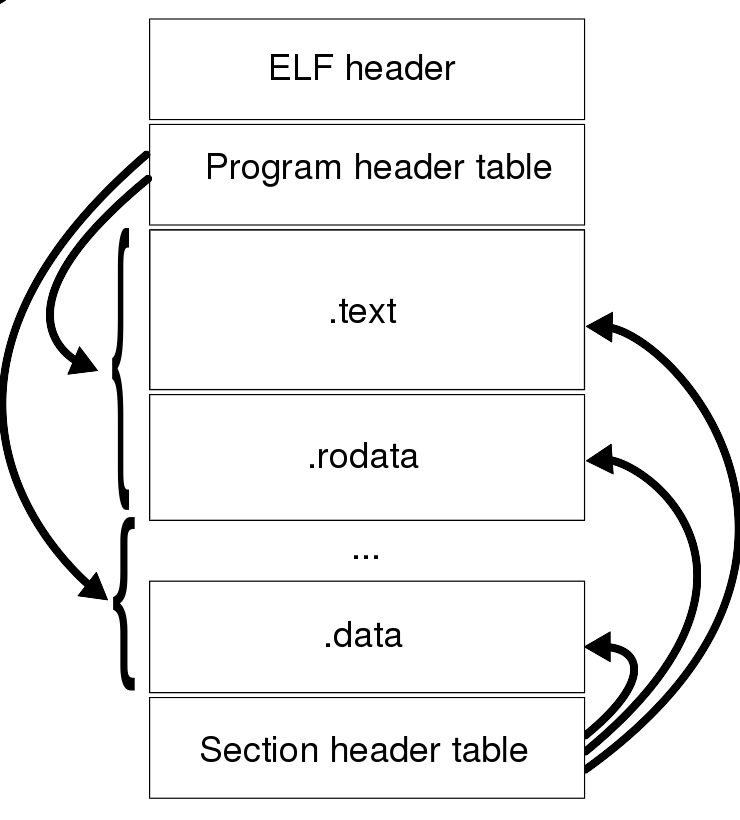
\includegraphics[width=6cm]{pictures/elf_layout}
\end{center}
\label{fig:elf}
\caption{Architecture d'un binaire ELF}
\end{figure}

\paragraph{}
Parmi les diff�rentes sections, on retrouve:
\begin{itemize}
\item La section {\texttt .text}, contenant le code ex�cutable
\item La section {\texttt .data}, contenant les donn�es accessibles en �criture. Il peut s'agir de variables globales
par exemple.
\item La section {\texttt .ro-data}, contenant les donn�es accessibles en lecture seule. Il s'agit
entre autres des cha�ne de caract�res {\it brutes}, comme la variable suivante :\\
\begin{lstlisting}
char    ma_version="version 1.0.2rc3";
\end{lstlisting}
\end{itemize}

\paragraph{}
Les sections qui ne figurent pas dans un binaire sont les sections {\it dynamiques}, construites du
fait de l'ex�cution du logiciel. Il s'agit du tas (heap) et de la pile (stack). Ces   sections
sont sp�cifiques au processus\footnote{Un processus est une tache {\it en cours d'ex�cution}, �
l'inverse d'un ex�cutable, qui n'est qu'un fichier}.

\paragraph{}
Lors du linkage, on ne retrouve plus qu'une seule section de code (section .text). Elle regroupe l'ensemble des
sections de code des fichiers objets. Du fait du regroupement, les offset des diff�rents symboles d�finis dans les
fichiers objets changent en fonction de leur position dans la nouvelle section .text. Il s'agit de la premi�re
translation des adresses des symboles. La seconde s'effectue durant l'ex�cution du processus associ� au binaire, en
fonction de son positionnement dans l'espace m�moire virtuel.

\section{Qu'en est-il de l'emploi des biblioth�ques tierces ?}

\paragraph{}
Lors de l'impl�mentation d'un logiciel, on fait souvent appel � des biblioth�ques tierces. La premi�re, dans le cas
du C, est la biblioth�que GNU Libc. En C++ il s'agit de la libstdC++ et r�guli�rement de boost. Il existe de
nombreuses autres biblioth�ques, sp�cialis�es chacune dans un domaine, comme la libxml, la libgtk ou encore la
libdvdread.

\paragraph{}
Il y a deux mani�res de prendre en compte les biblioth�ques lors de la  construction  d'un  binaire:
\begin{enumerate}
\item On int�gre le code de la biblioth�que dans le binaire. Dans ce cas, les symboles de la biblioth�que sont
int�gr�s comme autant de nouveaux symboles dans la table des symboles du binaire. Le code des fonctions de la
biblioth�que est  int�gr�  quant  �  lui  dans  la   section   {\texttt   .text}   du   binaire.\\
Il faut prendre note toutefois que le linker, loin d'�tre b�te, n'ajoute que le code de la biblioth�que n�cessaire
� l'ex�cution du binaire. Les symboles n'�tant pas appell�s directement ou indirectement dans le binaire ne sont pas
int�gr�s. Cela a un impact lors de la gestion des options de linkage durant la phase de compilation. Il s'agit d'une
des erreurs commun�ment faites si l'on n'y pr�te pas garde.

\item On maintient les symboles comme �tant non r�solus, et c'est le noyau, lors de la cr�ation du processus, qui va
mapper en m�moire la biblioth�que. L'int�r�t principal est de partager les ressources entre les divers processus.
En effet, en consid�rant le cas de la libc, des centaines de processus s'en servent. Plut�t que chacun emporte une
copie du code en son sein, ce dernier n'est pr�sent qu'une fois en m�moire, et est partag� entre les diff�rents
processus.\\
Le premier processus � s'en servir mappe r�ellement la biblioth�que en m�moire, et les autres processus, par un jeu
de mappage multiple des pages de code de la biblioth�que (au travers de la MMU) acc�dent au final � la m�me adresse
physique.
\end{enumerate}

\section{Les options de la cha�ne de compilation}

\paragraph{}
Au travers de la commande {\tt gcc} sont ex�cut�s � la fois le pr�processeur ({\tt cpp}), le compilateur ({\tt gcc})
et le linker ({\tt ld}). En cons�quence, on fournit � gcc � la fois des options pour le preprocessing, pour la
compilation et pour le linkage.

\paragraph{}
Dans le cadre de ce document, le but est de d�crire les principales options et � quoi elles servent. Le manuel de gcc
d�crit tr�s bien les options par famille et par type. Il ne faut pas h�siter � s'appuyer dessus. Lorsque l'on cherche
plus particuli�rement les options de preprocessing ou de linkage, il vaut alors mieux s'appuyer sur le manuel
respectivement de cpp et de ld.

\paragraph{}
Tout d'abord, les options de preprocessing sont peu nombreuses et les conna�tre n'est pas une obligation. Sont
d�crites    ici    majoritairement    les    options    de    compilation,    puis    de    linkage.

\subsection{Les options de compilation}

\paragraph{}
Le tableau \ref{tab:gcc_flags} d�crit les option du compilateur GNU gcc.

\begin{table}
\begin{tabular}{|l|l|}
\hline
Option & Signification \\
\hline
\hline
{\textbf{-c}} &
        \begin{minipage}{0.7\linewidth}
        \vspace{2mm}
        Gcc g�n�re un fichier objet. Seule l'�tape de compilation, et au besoin de preprocessing sont ex�cut�es.
        \vspace{2mm}
        \end{minipage}\\
        \hline
%%%%%%%%%%%%%%%%%%%
{\textbf{-s}} &
        \begin{minipage}{0.7\linewidth}
        \vspace{2mm}
        Gcc g�n�re un fichier assembleur. Selon les options d'optimisation, le compilateur peut g�n�rer un code
        assembleur peu repr�sentatif du code du langage de haut niveau. C'est l� qu'on se rend compte de la
        complexit� des �lements de parsing et d'optimisation du code.
        \vspace{2mm}
        \end{minipage}\\
        \hline
%%%%%%%%%%%%%%%%%%%
{\textbf{-o}} &
        \begin{minipage}{0.7\linewidth}
        \vspace{2mm}
        Sp�cifie le nom du fichier de sortie du traitement � effectu�. Ainsi si l'option -c est donn�e le fichier de
        sortie est le fichier objet.
        \vspace{2mm}
        \end{minipage}\\
        \hline
%%%%%%%%%%%%%%%%%%%
{\textbf{-W}} &
        \begin{minipage}{0.7\linewidth}
        \vspace{2mm}
        Cette option demande au compilateur d'afficher les warnings les plus fr�quents. Cette option ne fait
        qu'afficher sur la sortie d'erreur ({\tt stderr}) les �l�ment de programmation hasardeux les  plus  graves.
        \vspace{2mm}
        \end{minipage}\\
        \hline
%%%%%%%%%%%%%%%%%%%
{\textbf{-Wall}} &
        \begin{minipage}{0.7\linewidth}
        \vspace{2mm}
        Idem � {\tt -W}, mais prend en compte plus de Warnings. Il regroupe un sous-ensemble des diff�rents
        warning  g�r�  par  gcc  (confer  le  manuel  de  gcc ({\tt man gcc}),   partie   {\it
        Warning   Options}).
        \vspace{2mm}
        \end{minipage}\\
        \hline
%%%%%%%%%%%%%%%%%%%
{\textbf{-Werror}} &
        \begin{minipage}{0.7\linewidth}
        \vspace{2mm}
        Demande au compilateur de s'arr�ter la compilation au premier warning d�cel�. Cette option est
        malheureusement rarement utilis�e
        \vspace{2mm}
        \end{minipage}\\
        \hline
%%%%%%%%%%%%%%%%%%%
{\textbf{-ansi}} &
        \begin{minipage}{0.7\linewidth}
        \vspace{2mm}
        Le compilateur v�rifie la conformit� du code au langage C ANSI. Dans le cas contr�re, il renvoie un Warning.
        \vspace{2mm}
        \end{minipage}\\
        \hline
%%%%%%%%%%%%%%%%%%%
{\textbf{-Wextra}} &
        \begin{minipage}{0.7\linewidth}
        \vspace{2mm}
        V�rifie un maximum de fragilit�s dans le code. Ce drapeau int�gre la quasi-totalit� des warnings support�s
        par gcc (pas tous !).
        \vspace{2mm}
        \end{minipage}\\
        \hline
%%%%%%%%%%%%%%%%%%%
{\textbf{-Wwrite-strings}} &
        \begin{minipage}{0.7\linewidth}
        \vspace{2mm}
        Le compilateur v�rifie qu'� aucun moment il y a �criture sur une cha�ne brute (�l�ment de la section {\texttt
        .rodata}, ne pouvant �tre r��crit).
        \vspace{2mm}
        \end{minipage}\\
        \hline
%%%%%%%%%%%%%%%%%%%
{\textbf{-g}} &
        \begin{minipage}{0.7\linewidth}
        \vspace{2mm}
        Lors de la compilation, int�grer les �l�ments de debug. Cela permet, lors du debugging de l'application durant
        son ex�cution, de pouvoir s'appuyer sur les symboles et les m�tainformations (nom r�el des fonctions, etc.).
        Dans le cas contraire, m�me le nom des fonctions (qui ne sont en fin de compte que des
        adresses) n'est pas pr�sent dans le binaire.
        \vspace{2mm}
        \end{minipage}\\
        \hline
%%%%%%%%%%%%%%%%%%%
{\textbf{-ggdb}} &
        \begin{minipage}{0.7\linewidth}
        \vspace{2mm}
        Les symboles de debug sont optimis�s pour gdb. Les informations sont plus grandes car mieux exploit�es par le
        debuggeur de la GNU.
        \vspace{2mm}
        \end{minipage}\\
        \hline
%%%%%%%%%%%%%%%%%%%
\end{tabular}
\label{tab:gcc_flags}
\caption{Options les plus courantes du compilateur}
\end{table}

\paragraph{}
Comme le tableau \ref{tab:gcc_flags} en montre un aper�u, il existe un grand nombre d'options de compilation. Il
n'est ici pr�sent� que les principales, mais en r�alit�, ma�triser ne serait-ce que la moiti� de ces options demande
plusieurs ann�es de d�veloppement.

\paragraph{}
Fort heureusement, l'�tape de compilation est la plus riche en terme d'option, et l'�tape de linkage n�cessite moins
de connaissance.\\
Cependant, la compr�hention pouss�e du principe de fonctionnement du linkage est tr�s importante car elle est � la
base de la compr�hention de l'usage de la m�moire par les processus, et par extention de son impact sur ses
performances et sur sa s�curit�.

\paragraph{}
Enfin, il est important de noter que de nouvelles options de compilation apparaissent au fur et � mesure des nouvelles
versions de gcc. Avec un bon usage de ces options, on r�duit fortement le risque de bug durant l'ex�cution du
logiciel.


\subsection{Les options de linker}

\paragraph{}
Seules   deux   options   de   linkage   sont    d�crites    dans    le    tableau    \ref{tab:ld_opts}
\begin{table}
\begin{tabular}{|l|l|}
\hline
Option & Signification \\
{\textbf{-l}} &
        \begin{minipage}{0.7\linewidth}
        Informe le linker que le logiciel � linker s'appuie sur une biblioth�que ext�rieure au logiciel. Cette option
        est implicite pour la libc, mais doit �tre fournie pour toutes les autres biblioth�ques. Seul le nom de la
        biblioth�que,   sans   le   prefixe   {\it   lib}   doit   �tre   fourni.     Voici un
        exemple avec la libgtk (biblioth�que graphique sur laquelle se base le bureau Gnome) :\\
        \begin{lstlisting}
        gcc -o foo -lgtk foo.c
        \end{lstlisting}
        \end{minipage}\\
        \hline
%%%%%%%%%%%%%%%%%%%
{\textbf{-L}} &
        \begin{minipage}{0.7\linewidth}
        Il arrive que la biblioth�que utilis�e ne soit pas pr�sente dans les r�pertoires par d�faut des biblioth�ques
        ({\texttt /lib, /usr/lib} et {\texttt /usr/local/lib}). Il faut alors pr�ciser au linker o� se situe la
        biblioth�que.  Cette option prend  en  argument  le  chemin  absolu  vers  la  biblioth�que.
        \end{minipage}\\
        \hline
%%%%%%%%%%%%%%%%%%%
\end{tabular}
\label{tab:ld_opts}
\caption{Options de base du linker}
\end{table}


%%
%%
%% makefiles.tex for  in /doctorat/ece/partenariat/cours/outils_gnu
%%
%% Made by Philippe THIERRY
%% Login   <Philippe THIERRYreseau-libre.net>
%%
%% Started on  Wed Sep  1 18:07:34 2010 Philippe THIERRY
%% Last update dim. 12 sept. 2010 11:44:36 CEST Philippe THIERRY
%%

\chapter{La commande GNU Make}

% style for Makefile
\lstset{
morecomment=[l][\color{blue}]{\#},
morekeywords={include,ifeq,ifneq,ifndef,ifdef,else,endif,.c.o}
%morecomment=[s][\color{green}]{\$(}{)},
emph={[2].PHONY},emphstyle={[2]\color{red}}
}



{\it Il s'agit, dans le cadre de ce chapitre, de d�crire comment on automatise la production de
gros logiciels, et quelles sont les probl�matiques qui en d�coulent}

\section{Principe des \index{Makefile}Makefiles}

\paragraph{}
Le syst�me de Makefile a �t� cr�� dans le but de simplifier la production d'un logiciel. Il
s'articule autour de fichiers de configuration, nomm�s {\tt Makefile}, qui d�finissent les
diff�rents �l�ments des sources et le traitement qui leur est associ�.\\
Ces fichiers de configuration sont trait�s par le binaire {\tt make}, qui existe en plusieurs
versions, dont les c�l�bres BSD Make et GNU Make. Sous Linux, c'est le make de la GNU qui est
install� par d�faut. Cette version int�gre des capacit�s suppl�mentaires par rapport au make de BSD,
ce qui peut parfois rendre les Makefiles non portables s'ils utilisent ces fonctionnalit�s.

\subsection{Les cibles et les d�pendances}

\paragraph{}
Dans un fichier Makefile, on appelle {\it cible} (target) un ensemble de traitements r�unis sous un
m�me nom.\\
Cette cible est appellable comme argument de la commande {\tt make}, impliquant l'ex�cution de
la cible demand�e :
\begin{lstlisting}[caption={Appeler une cible sp�cifique dans un Makefile},label=lst:call_target]
sh$ make -j 2 ma_cible
\end{lstlisting}

\paragraph{}
Un cible de Makefile se r�dige ainsi:
\begin{lstlisting}[caption={R�daction d'une premi�re cible de Makefile},label=lst:mak_target]
ma_cible:
	echo "executing ma_cible"
	cp fichier1 fichier2
	echo "end of execution of ma_cible"
\end{lstlisting}

\paragraph{}
Le nom d'une cible doit �tre �crit en un seul mot, et doit �tre imp�rativement seul avant les
deux points. Il est possible de lui pr�ciser des d�pendances apr�s les deux points, comme un
ensemble d'autres cibles qui seront appell�es dans l'ordre d'�criture.

\paragraph{}
Tous les traitements ex�cut�s par une cible s'�crivent en commen�ant par le caract�re tabulation,
et doivent se succ�der sans ligne blanche ou tout autre ligne ne commen�ant pas par une
tabulation.\\
Une ligne blanche indique la fin de la cible en cours.

\paragraph{}
Comme dit pr�c�demment, une cible peut avoir des d�pendances envers d'autres cibles. Cela s'�crit
simplement comme une suite de cibles � droite des deux points:
\begin{lstlisting}[caption={D�finir des d�pendances entres cibles de Makefile},label=lst:mak1]
prepare:
	touch fichier1

get_info:
	cat /proc/cpuinfo > fichier1

ma_cible: prepare get_info
	echo "executing ma_cible"
	cp fichier1 fichier2
	echo "end of execution of ma_cible"
\end{lstlisting}

\paragraph{}
En demandant l'ex�cution de la cible {\it ma\_cible}, la commande make va successivement ex�cuter,
dans cet ordre, les cibles {\it prepare}, {\it get\_info}, et {\it ma\_cible}.

\paragraph{}
Comme on le voit dans cette section, le syst�me de Makefile ne sert pas uniquement � automatiser la
compilation. Il est capable d'ex�cuter n'importe quelle commande.

L'usage d'un Makefile tel que dans le script \ref{lst:mak1} est assez simpliste. Il est en r�alit�
possible de cr�er des Makefiles beaucoup plus complexes en s'appuyant compl�tement sur la grammaire
de make.

\section{Le langage des Makefiles}

\subsection{Les variables}

\paragraph{}
Dans un Makefile, il est possible de d�finir des variables. La d�finition d'une variable se fait
par convention avant la d�finition des r�gles. Ces derni�res peuvent alt�rer la valeur d'une
variable en fonction du besoin.

\paragraph{}
Une variable de Makefile s'�crit par convention en majuscule. Sa d�finition peut se faire de trois
mani�res, comme l'indique le script \ref{lst:makvar}.

\begin{lstlisting}[caption={Les variables dans les Makefiles},label=lst:makvar]
VAR = foo
VAR ?= foo
VAR += foo
\end{lstlisting}

\paragraph{}
Les trois mani�res d'assigner une valeur � une variable sont, dans l'ordre d'apparition :
\begin{enumerate}
\item la variable {\it VAR} vaut {\tt foo}
\item la variable {\it VAR} vaut {\tt foo} uniquement si elle n'existe pas d�j�. Si cette derni�re
est d�j� existante dans le contexte d'ex�cution du Makefile, elle n'est pas modifi�e.
\item la variable {\it VAR} voit sa valeur concat�n�e avec la valeur en argument, un espace
s�parant les deux valeurs.
\end{enumerate}

\paragraph{}
Il est possible d'assigner � une variable le r�sultat d'une ligne de commande. Pour cela, on
encapsule la valeur dans le marqueur {\tt \$()}.

\begin{lstlisting}[caption={Assigner le r�sultat d'une commande � une variable},label=lst:cmd_var]
DATE = $(date +"%d-%M-%Y")
\end{lstlisting}

\subsection{Les structures de contr�le}

\paragraph{}
Il existe des structures de contr�le dans le langage des Makefiles. Elles permettent de ne
faire prendre en compte, par l'outil {\tt make}, qu'une partie du Makefile en fonction de la valeur
d'une donn�e. Cela permet, par exemple, de faire d�pendre un traitement d'un �l�ment ext�rieur.

\begin{lstlisting}[caption=Les structures de contr�les des Makefiles,label=lst:mak_ctrl]
CFLAGS=-W -ggdb

ifeq ($(MORE_CFLAGS),1)
	CFLAGS += -Wall -Wextra -Werror
endif

compile:
	gcc $CFLAGS) my_file.c -o foo

\end{lstlisting}

\paragraph{}
Le script \ref{lst:mak_ctrl} peut donc g�n�rer deux appels au compilateur. Un appel classique �
{\tt make compile} ex�cute la commande suivante :\\
\begin{lstlisting}
gcc -W -ggdb my_file.c -o foo
\end{lstlisting}
� l'inverse, la commande {\tt MORE\_CFLAGS=1 make compile} ex�cute la commande suivante :
\begin{lstlisting}
gcc -W -ggdb -Wall -Wextra -Werror my_fyle.c -o foo
\end{lstlisting}

\paragraph{}
Dans le cadre du script \ref{lst:mak_ctrl}, c'est l'assignation d'une variable qui est encadr�e. Il
est cependant possible d'utiliser les structures de contr�le pour encapsuler des cibles enti�res,
en fonction du besoin.

\paragraph{}
Il existe d'autres structures de contr�le dans le langage des Makefiles. Il s'agit des
d�clarations:\\
\begin{itemize}
\item {\tt ifneq-else-endif}, qui se base sur un test faux d'�galit�
\item {\tt ifdef-else-endif}, qui se base sur l'existance de l'argument
\item {\tt ifndef-else-endif}, qui se base sur la non-existance de l'argument
\end{itemize}


\subsection{La r�cursivit�}

\paragraph{}
Comme vu pr�c�demment, les sources d'un projet contiennent plusieurs r�pertoires. Par convention, un
Makefile donn� ne traite que du r�pertoire dans lequel il est pr�sent. Ainsi, on r�dige non pas un
seul mais plusieurs Makefiles, avec un seul Makefile dit {\it racine}, se chargeant d'appeller les
autres en fonction du besoin.

\paragraph{}
\begin{lstlisting}[caption=R�partition des Makefiles dans un projet,label=lst:mak_directory]
 [d] doc/
  f     Makefile
  f     mydoc.tex
 [d] src/
  f     Makefile
  f     foo.c
  f AUTHORS
  f ChangeLog
  f Makefile
  f README
\end{lstlisting}

\paragraph{}
Par convention, le Makefile se trouvant � la racine du r�pertoire est dit Makefile {\it racine}.
C'est lui qui se chargera d'appeller les autres Makefiles en fonction du besoin. En effet, le
d�veloppeur, et plus g�n�ralement l'utilisateur du logiciel, n'a pas � conna�tre la d�composition des
sources du logiciel pour le construire. Seules les commandes fournies par le Makefile de la racine
doivent suffire � compiler l'ensemble. En consid�rant le r�peroire projet
\ref{lst:mak_directory}, le Makefile de la racine serait proche de celui donn� dans le script
\ref{lst:root_mak}\\

\begin{lstlisting}[caption={Makefile racine type},label=lst:root_mak]
all:
	make -C src all

doc:
	make -C doc all

help:
	echo "make all compile les sources, make doc g�n�re la documentation"
\end{lstlisting}

\paragraph{}
L'option -C de make permet de lui sp�cifier dans quel r�pertoire il doit chercher le Makefile. On
constate donc qu'en ex�cutant la commande {\tt make all} � la racine, cette derni�re va, par
r�cursion, appeller la commande {\tt make all} dans le r�pertoire src.\\
Il en va de m�me pour la commande {\tt make doc} qui va appeller la commande {\tt make all}, dans
doc.

\subsection{Construire des �l�ments communs � tous les Makefile}

\paragraph{}
Il arrive qu'un certain nombre d'�l�ments puissent �tre redondants parmis les diff�rents Makefiles.
Il peut s'agir de variables ou de cibles. Plut�t que de r��crire ces �l�ments dans chaque Makefile
avec un risque d'inconcistance, il est possible d'�crire un sous-ensemble du Makefile dans un
fichier qui sera int�gr� dans les diff�rents Makefiles du projet.

\paragraph{}
Par convention, ces Makefiles ont une extention de fichier {\tt .mk}. Il n'y a pas de convention
sur leur nom et peuvent �tre appell�s de diff�rentes mani�res.

\paragraph{}
Afin d'inclure un (ou plusieurs) de ces fichiers dans un Makefile, on utilise la directive {\tt
include}.
Le script \ref{lst:mak_mk} est un exemple de fichier {\tt .mk}.

\begin{lstlisting}[caption={Exemple de fichier .mk : infos.mk},label=lst:mak_mk]
PROJECTVERSION=0.12.3
PROJECTNAME=libfoobar
AUTHOR="Dave Null"
\end{lstlisting}

Le script \ref{lst:mak_include} donne un exemple de ligne d'inclusion d'un tel fichier.

\begin{lstlisting}[caption={Inclusion d'un fichier mk dans un Makefile},label=lst:mak_include]
include infos.mk

PROJDIR=$(PROJECTNAME)-$(PROJECTVERSION)

init:
	mkdir $(PROJDIR)
	@echo $(AUTHOR) > $(PROJDIR)/Authors

...
\end{lstlisting}


\section{D�composer et automatiser la compilation}

\paragraph{}
Il a �t� vu pr�c�dement que le syst�me de Makefile fournit une base simple et efficace pour
automatiser des traitements, et ce de toute nature.\\
Cependant, l'�l�ment pour lequel les Makefiles prennent tout leur sens et fournissent le plus de
capacit�s est l'automatisation de la production. On parle bien ici de production et non simplement
de compilation, qui n'est en r�alit� qu'un de ses multiples aspects, avec la g�n�ration de docs,
l'ex�cution des campagnes de tests, ou encore l'installation de l'applicatif.

\subsection{La grammaire des Makefiles pour la compilation}

\paragraph{}
De mani�re g�n�rale, pour une r�gle donn�e, il existe deux variables importantes :
\begin{itemize}
\item {\tt \$@} : cette variable contient le nom de la r�gle courante, et peut donc �tre utilis�e
lors de la r�daction des actions d'une r�gle.
\item {\tt \$<} : cette variable contient le nom des �l�ments d'entr�e d'une r�gle. Cette variable
est r�guli�rement utilis�e dans la r�daction des cibles de compilation.
\end{itemize}

\paragraph{}
Un autre �l�ment tr�s utile des Makefiles est l'aspect traitement de cha�ne de caract�re lors de la
d�finition d'une variable, dont la syntaxe est ressemblante � celle du {\it bash}.\\
Ainsi, on peut, � partir d'une variable ayant une cha�ne de caract�re donn�e, la modifier comme on
le souhaite pour d�finir d'autres variables. Un exemple �tant toujours mieux qu'un long discours,
voici un exemple d'emploi permettant, pour une cha�ne donn�e, de remplacer une sous-cha�ne par une
autre :\\
\begin{lstlisting}[caption={Traitement de cha�nes de caract�res dans les Makefiles},label=lst:mak_glob]
SOURCE = main.c
OBJ = $(SOURCE:.c=.o) # ici, OBJ vaut main.o
ASM = $(SOURCE:.c=.s) # ici ASM vaut main.s
\end{lstlisting}

L'int�r�t principal est de d�finir la cha�ne � un seul endroit, pour en d�river sa valeur ensuite.
Cela permet d'�viter une inconsistance en d�finissant plusieurs fois la cha�ne compl�te.

\subsection{Les variables de compilation}

\paragraph{}
Il existe un certain nombre de variables r�guli�rement utilis�es pour r�diger un Makefile pour la
compilation. Ces derni�res sont celles employ�es par les outils de configuration des sources. Sont
d�crites ici les variables associ�es � des projets �crits en C ou en C++.

\begin{itemize}
\item CFLAGS : d�finit les options de compilation pour un programme en C
\item CXXFLAGS : d�finit les options de compilation pour un programme en C++
\item LDFLAGS : d�finit les options de linkage pour un programme en C ou C++
\item TARGET : d�finit le nom du binaire produit par les sources
\item SOURCES : liste les fichiers sources du projet
\item OBJECTS : liste les fichiers objets du projet
\item HEADERS : liste les en-t�tes du projet
\item CC : le compilateur C, en chemin relatif ou absolu
\item CXX : le compilateur C++, en chemin relatif ou absolu
\item LD : le linker, en chemin relatif ou absolu
\item AS : l'assembleur, en chemin relatif ou absolu
\end{itemize}

\paragraph{}
Il existe d'autres variables, mais les principales sont d�finies ici. On en retrouve une liste plus
grande dans le script \ref{lst:mak_all}.

\subsection{Les subtilit�s des nom de cibles}

\paragraph{}
Il est tout � fait possible d'utiliser une variable comme nom de cible. C'est d'ailleurs souvent le cas
comme le montre le script \ref{lst:mak_all}.

\paragraph{}
Il existe de plus des noms de cibles sp�cifiques. Il en existe un particulier pour la compilation.
Afin d'en comprendre le sens, voici son usage:
\begin{lstlisting}
.c.o :
	$(CC) $(CFLAGS) -c $<
\end{lstlisting}
Cette cible est faite pour la compilation des fichiers sources en fichiers objets. Cette r�gle
prend en entr�e les fichiers se terminant par l'extension {\tt .c} d�finis plus haut dans le
Makefile et les int�gre � la variable {\tt \$<} pour pouvoir �tre utilis�s.\\
Dans le script \ref{lst:mak_all}, cette r�gle est utilis�e pour g�n�rer les fichiers objets �
partir des sources. L'ensemble des fichiers sources sont int�gr�s � la variable {\tt \$<} qui est
utilis�e dans la r�gle �crite pour cette cible.

\subsection{Les r�gles PHONY}
\index{Makefile!PHONY}

\paragraph{}
Il arrive parfois qu'un fichier ou un dossier du r�pertoire courant porte le m�me nom qu'une cible.
C'est en g�n�ral le cas de {\it doc}.\\
Le probl�me est que le syst�me de Makefile consid�re que si le nom d'une cible porte le nom d'un
fichier ou d'un r�pertoire, ce dernier est la cons�quence de la cible elle-m�me. En cons�quence, si
ce dernier est pr�existant lors de l'appel � cette cible et que cette derni�re ne poss�de pas de
d�pendance, alors elle ne sera pas ex�cut�e.\\
Dans l'exemple d'une cible {\tt doc}, o� le r�pertoire doc est d�j� pr�sent dans le r�pertoire
courant, on a le comportement suivant:
\begin{lstlisting}
sh$ make doc
target 'doc' already up to date.
sh$
\end{lstlisting}
Afin de forcer l'ex�cution de la cible m�me si le fichier/dossier est pr��xistant, on utilise la
cible sp�ciale {\it .PHONY}. Cette cible force l'ex�cution des cibles dont elle d�pend. Il y en a
un exemple dans le script \ref{lst:mak_all}.

\subsection{Un Makefile complet pour la compilation}

\paragraph{}

\begin{lstlisting}[caption={Exemple de Makefile complet pour la compilation},label=lst:mak_all]
#############################################################################
## basic macros
#############################################################################
CC          ?= gcc
AR	     = ar
CFLAGS      ?= -Wall -W -Werror -Wextra -ansi -pedantic
LD           = ld
LDFLAGS	     = 
ARFLAGS	     = cr
RM	     = rm
RMFLAGS      = -rf
TAR          = tar
TARFLAGS     = -cjvf
MAKE        ?= make
INSTALL      = install
CTAGS        = ctags -x > tags
DEPEND       = makedepend $(CFLAGS)
MAKE         = make

#############################################################################
## lint -- static code mistakes detector
#############################################################################
LINT         = splint
LARCH_PATH   = /usr/local/lib
LCLIMPORTDIR = /usr/local/share/splint/imports

#############################################################################
## dist target file
#############################################################################
DISTTARGET   = .tar.bz2

#############################################################################
## project's source and generated files
#############################################################################
TARGET	     = foobar
SOURCE	     =	main.c \
		foo.c \
		bar.c \
		baz.c

OBJS	     = $(SOURCE:.c=.o)
HEADERS      = $(SOURCE:.c=.h)
TODEL	     = tags *~ .*.swp

#############################################################################
## rules
#############################################################################

all : $(TARGET)

$(TARGET) : $(OBJS)
	$(CC) -o $@ $(OBJS) $(LDFLAGS)

.c.o :
	$(CC) $(CFLAGS) -c $<

doc :
	$(MAKE) -C doc all

lint :
	$(LINT) $(CFLAGS) $(SOURCE)

tags : $(SOURCE)
	$(CTAGS) $(SOURCE)

depend : $(SOURCE)
	$(DEPEND) $(SOURCE)

.PHONY : clean doc

clean : 
	$(RM) $(RMFLAGS) $(OBJS) $(TODEL)

distclean : clean
	$(RM) $(RMFLAGS) $(TARGET)

dist : distclean
	$(TAR) $(TARFLAGS) $(DISTTARGET) .

check : $(TARGET)
	cd check; $(MAKE) all

install : $(TARGET)
	@echo you must be root to install
\end{lstlisting}

\section{Les limitations}

\paragraph{}
Le syst�me de Makefile poss�de un certain nombre de limitations et de probl�matiques. En premier
lieu, il ne permet pas, de mani�re ais�e, de v�rifier les capacit�s de la cha�ne de compilation.
Ainsi, lorsque l'on d�finit certaines variables comme CFLAGS, on prend comme hypoth�se que la
cha�ne de compilation les reconna�t.\\
Cependant, en faisant ainsi, on se heurte parfois � des probl�mes de portabilit�. En effet, il
arrive fr�quemment que le projet soit compil� avec une cha�ne de compilation dont on ne ma�trise pas
les versions du compilateur ou encore du linker. Ainsi, selon la version utilis�e, les options de
compilation d�finies dans le Makefile peuvent ne pas �tre reconnues, et provoquer un arr�t de la
construction du projet.\\
Il en va de m�me pour la v�rification de la pr�sence des divers binaires n�cessaires � la
production. Il est possible de d�finir des fonctions de v�rification dans le Makefile, mais elles
sont � �crire par l'utilisateur et peuvent �tre nombreuses. C'est pour cette raison qu'on utilise
souvent, en compl�ment du syst�me de Makefiles, un syst�me de configuration, comme les {\it
autotools}\index{autotools} ou encore {\it CMake}\index{CMake}.\\
Les autotools �tant le plus fr�quemment utilis�s (ils sont � l'origine de la commande {\tt
configure} que l'on ex�cute r�guli�rement lors de l'installation d'un applicatif � partir de ses
sources) car plus anciens. Ce document s'int�resse dans le chapitre suivant � leur fonctionnement
g�n�ral.

%%
%%
%% les_outils_de_conf.tex for  in /doctorat/ece/partenariat/cours/outils_gnu
%%
%% Made by Philippe THIERRY
%% Login   <Philippe THIERRYreseau-libre.net>
%%
%% Started on  Wed Sep  1 18:07:52 2010 Philippe THIERRY
%% Last update dim. 12 sept. 2010 12:14:39 CEST Philippe THIERRY
%%

\chapter{Les outils de configurations des sources}
\label{chap:autotools}

{\it Ce chapitre parle des diff�rents outils permettant de combler les limitations du syst�me de
Makefiles.\\
L'outil qui sera abord� sera le syst�me d'autotools, car il est le plus commun�ment
employ�}

\section{Pourquoi configurer ses sources ?}

\paragraph{}
La production d'un logiciel n�cessite un certain nombre de biblioth�ques et d'outils dont il est
plus prudent d'en v�rifier la pr�sence avant la production effective. De m�me, il peut �tre
n�cessaire, dans certains cas, de v�rifier les capacit�s des outils de compilation afin de
d�terminer les options qu'il faut leur fournir.\\
Ce type de v�rification, bien que faisable dans le cadre d'un Makefile, n'est pas pr�vu pour �tre
simplifi� ou automatis�. C'est l� qu'interviennent les outils de configuration des sources et du
syst�me de production, permettant de fournir aux Makefiles toutes les informations n�cessaires au
bon fonctionnement de la production.\\
Un autre point non pris en compte par les Makefiles est le processus de packaging. Il s'agit de
pouvoir construire de mani�re simple une archive, dans un format le plus g�n�rique possibe (en
g�n�ral il s'agit du format {\tt .tar.gz}, support� par toute installation minimum d'un Linux ou
d'un unix (*BSD par exemple) et compatible de toutes les plateformes embarqu�es).\\
Cette archive doit �tre autosuffisante : il ne doit rien lui manquer pour pouvoir construire le
logiciel associ�, du moment que les outils de production sont pr�sents.

\paragraph{}
Un exemple simple est celui de la construction de la documentation. Comme vu dans le chapitre
pr�c�dant, il existe r�guli�rement une cible {\tt doc} dans le Makefile racine, permettant de
construire la documentation.\\
Cette documentation est parfois r�dig�e en \LaTeX, ce qui implique la pr�sence du compilateur LaTeX
et les biblioth�ques associ�es. Ces outils ne sont pas n�cessairement pr�sents sur une installation
Linux standard, et il devient important de v�rifier leur pr�sence afin de fournir � l'utilisateur un
message compr�hensible lui demandant de les installer. A d�faut, le Makefile produira un message de
type {\tt file not found} et renverra une erreur, pas forc�ment simple � lire.


\section{Les limites de la configuration : probl�matique de la cross-compilation}

\paragraph{}
Le syst�me de configuration est capable de fournir un grand nombre d'informations. Le tableau
\ref{tab:config_info} donne une liste d'�l�ments que ce dernier peut fournir en entr�e de la
production.

\begin{table}
\begin{tabular}{|l|}
\hline
{\it Informations r�cup�rables par l'outil de configuration des sources}\\
\hline
\hline
La version du compilateur, du pr�processeur, du linker \\
\hline
Les options que supporte le compilateur, le pr�processeur, le linker \\
\hline
La taille d'un integer, d'un long, d'un double, d'un pointeur \\
\hline
La pr�sence de divers headers du langage de programmation du projet \\
\hline
Pour une biblioth�que donn�e, la pr�sence de diverses fonctions du langage de programation du projet \\
\hline
La pr�sence de tout binaire demand� \\
\hline
des valeurs de CFLAGS, LDFLAGS personnalis�es en fonction des informations trouv�es \\
\hline
des �l�ments de configuration pour la production et l'installation du binaire (emplacement, etc) \\
\hline
\end{tabular}
\caption{Les informations fournies par l'outil de configuration des sources}
\label{tab:config_info}
\end{table}

\paragraph{}
Parmi toutes les capacit�s du syst�me de configuration, certaines ne sont pas n�cessairement bonnes
� utiliser. C'est entre autre le cas des informations sur la taille en octets des types num�riques.\\
En effet, lorsque l'on fait de la cross-compilation, c'est en g�n�ral sur une plateforme donn�e pour une
autre. Par exemple, on cross-compile sur une architecture Intel IA32 pour un processeur ARM.

\paragraph{}
Lorsque le syst�me de production r�cup�re les informations sur les tailles de type, il le fait sur
la plateforme locale, non sur la plateforme cible. Il n'a d'ailleurs aucune possibilit� de
conna�tre,  au moment de la compilation, les propri�t�s de la plateforme cible. Ainsi, on consid�re
qu'un syst�me de configuration des sources ne doit aider que pour v�rifier les �l�ments n�cessaires �
la production, en aucun cas � l'ex�cution. On va donc v�rifier la pr�sence des diff�rents binaires,
headers et fonctions n�cessaires � la compilation, et on laissera au d�veloppeur le soin
d'impl�menter son code de mani�re portable, sans avoir besoin de s'appuyer sur des informations que
pourrait lui fournir le syst�me de configuration lors de l'impl�mentation du logiciel.

\section{G�n�ralit�s sur la structure des autotools}

\subsection{Le fichier configure.ac}

\paragraph{}
Le fichier {\tt configure.ac} est au c{\oe}ur de la configuration des sources. C'est dans ce fichier qu'on
d�clare le nom du projet, sa version, la structure des sources, la position des diff�rents Makefiles
et les �l�ments que l'on souhaite faire v�rifier par le syst�me de configuration.\\
Le script \ref{lst:config_ac} est un exemple complet de fichier {\tt configure.ac}.

\begin{lstlisting}[caption={Fichier configure.ac typique d'un projet logiciel en C},label=lst:config_ac]
#############################################################################
# basic init                                                                #
#############################################################################
AC_INIT([libfoo], [0.98.7.rc2], [Philippe.thierry@ece.fr], [libfoo])

# version minimum des autotools
AC_PREREQ([2.61])
# type de projet, format de l'archive de sortie
AM_INIT_AUTOMAKE([1.9.5 foreign dist-bzip2 no-dist-gzip foreign])
# repertoire parent des sources C
AC_CONFIG_SRCDIR([src/libfoo.h])
# nom du fichier header ou les infos r�cup�r�es seront �crites
AM_CONFIG_HEADER(config.h)
# langage du projet
AC_LANG([C])

#############################################################################
# C specific standard verifications                                         #
#############################################################################
# verifier la compatibilite posix de la toolchain
AC_ISC_POSIX
# verifier le support du C
AC_PROG_CC
# verifier le support du C ANSI
AM_PROG_CC_STDC
# verifier la presence des headers pour le C ANSI
AC_HEADER_STDC
# verifie le support des mots clefs const, inline et volatile, ou suppression
# de ces mots clefs lors de la compilation
AC_C_CONST
AC_C_INLINE
AC_C_VOLATILE

#############################################################################
# Checking some basic headers and funcs                                     #
#############################################################################
AC_CHECK_HEADER([sys/types.h],,AC_MSG_ERROR([Cannot find sys/types.h ! Check your installation !]))
AC_CHECK_HEADER([ctype.h],,AC_MSG_ERROR([Cannot find ctype.h ! Check your installation !]))
AC_CHECK_HEADER([inttypes.h],,AC_MSG_ERROR([Cannot find inttypes.h ! Check your installation !]))
AC_CHECK_HEADER([errno.h],,AC_MSG_ERROR([Cannot find errno.h ! Check your installation !]))
AC_CHECK_HEADER([string.h],,AC_MSG_ERROR([Cannot find string.h ! Check your installation !]))
AC_CHECK_HEADER([sys/stat.h],,AC_MSG_ERROR([Cannot find sys/stat.h ! Check your installation !]))

# verification de l'accessibilite de certaines fonctions
AC_CHECK_FUNCS([strndup strncpy strdup strcat strcpy dup dup2 sigaction \
sigprocmask htons htonl snprintf sprintf fcntl])

# checking sizeofs (attention ! incompatible avec la cross compilation !)
AC_CHECK_SIZEOF([int])
AC_CHECK_SIZEOF([long])
AC_CHECK_SIZEOF([long long])
AC_CHECK_SIZEOF([double])
AC_CHECK_SIZEOF([int *])

#############################################################################
# Checking libraries presence                                               #
#############################################################################
AC_CHECK_LIB(m, powf, [], AC_MSG_ERROR([Cannot find libm match library ! Check your installation !]), [])

#############################################################################
# Support for compiler capacity to manage warning flags                     #
#############################################################################

# verification des flags supportes par le compilateur
# creation de la variable WARNING_CFLAGS en fonction de ce qui est supporte
LIBFOO_CC_WARNINGS([
                      [-Wall],
                      [-W],
                      [-Werror],
                      [-Wundef],
                      [-Wno-multichar],
                      [-Wextra],
                      [-Wtrigraphs],
                      [-Wundef],
                      [-Wswitch],
                      [-Wunused],
                      [-Wmissing-prototypes],
                      [-Wpacked],
                      [-Waggregate-return],
                      [-Wimplicit],
                      [-Wcast-qual],
                      [-Wcast-align],
                      [-Wwrite-strings],
                      [-Wuninitialized],
                      [-Winit-self],
                      [-fno-common],
                      [-pedantic],
                      [-Wshadow],
                      [-Wunsafe-loop-optimizations],
                      [-std=c99],
                      [-Wreturn-type],
                      [-Wimplicit-int],
                      [-Wmain],
                      [-Wcomment],
                      [-Wformat],
                      [-Wchar-subscripts],
                      [-Wimplicit-function-declaration],
                      [-Wchar-subscripts],
                      [-Wparentheses],
                      [-Wmissing-declarations],
                      [-Wredundant-decls],
                      [-Wstrict-prototypes],
                      [-Wnested-externs],
                      [-Wfloat-equal],
                      [-Wpointer-arith],
                      [-Wbad-function-cast],
                      [-Wsequence-point],
])

#############################################################################
# Support for static lib creation                                           #
#############################################################################
# demande d'utiliser libtool pour construire la bibliotheque libfoo.la
AC_PROG_LIBTOOL

############################################################################
# Checking needed softwares presence                                        #
#############################################################################
# demande d'utiliser l'utilitaire install pour la cible d'installation du projet
AC_PROG_INSTALL

# verification de la presence du binaire sloccount
AC_CHECK_PROG([SLOCCOUNT], [sloccount], [yes], [no])
if test X$SOCCOUNT = "X:"; then
  AC_MSG_WARN([Unable to detect sloccount in your path. You will not be able \
  to generate the SLOC counts.], 2)
  sloccount="no";
else
  sloccount="yes";
fi

# verification de la presence du binaire gprof
AC_CHECK_PROG([GPROF], [gprof], [yes], [no])
if test X$GPROF = "X:"; then
  AC_MSG_WARN([Unable to detect gprof in your path. You will not be able \
  to generate libcommon function calls profile.], 2)
  gprof="no";
else
  gprof="yes";
fi

# verification de la presence du binaire gcov
AC_CHECK_PROG([GCOV], [gcov], [yes], [no])
if test X$GCOV = "X:"; then
  AC_MSG_WARN([Unable to detect gcov in your path. You will not be able \
  to generate libcommon tests coverage.], 2)
  gcov="no";
else
  gcov="yes";
fi

# verification de la presence du binaire valgrind
AC_CHECK_PROG([VALGRIND], [valgrind], [yes], [no])
if test X$VALGRIND = "X:"; then
  AC_MSG_WARN([Unable to detect valgrind in your path. You will not be able \
  to generate dynamic memory usage in libcommon tests.], 2)
  valgrind="no";
else
  valgrind="yes";
fi

# verification de la presence du binaire latex
AC_CHECK_PROG([LATEX], [latex], [yes], [no])
if test X$LATEX = "X:"; then
  AC_MSG_WARN([Unable to detect latex in your path. You will not be able \
  to generate libcommon architecture documentation.], 2)
  latex="no";
else
  latex="yes";
fi

#############################################################################
# Checking specific arguments presence                                      #
#############################################################################
# support de l'option --with-efence, pour utiliser la bibliotheque Libefence
AC_ARG_WITH(efence, [  --with-efence           Link with electric fence ])
if test "$with_efence" = "yes"
then
	AC_CHECK_LIB(efence, EF_ALIGNMENT, LIBS="${LIBS} -lefence", AC_MSG_ERROR(libefence not found))
        efence="yes";
        EFENCE=1;
else
	efence="no";
fi

# support de l'option --with-debug, ajoutant les options de debug aux CFLAGS
AC_ARG_WITH(debug, [  --with-debug            Activate -g option of gcc and delete -DNDEBUG macro])
if test "$with_debug" = "yes"
then
	debug="yes";
        cppdebug=1;
        DEBUG="-g";
else
	debug="no";
        cppdebug=0;
        DEBUG="";
fi       
AC_DEFINE_UNQUOTED([HAVE_DEBUG], ${cppdebug}, [specify if the software has been configured in debug mode])

#############################################################################
# Generating CFLAGS...                                                      #
#############################################################################

# construction complete des CFLAGS, en fonction des resultats precedants
CFLAGS="$CFLAGS -O2 $DEBUG -DLINUX -D_XOPEN_SOURCE=600 -DMEMTRACE -std=c99 $WARNING_CFLAGS"

#############################################################################
# Finishing. Specify new conditionnals and Makfiles                         #
#############################################################################
# liste des Makefiles � generer � partir des fichiers Makefile.am (confer plus loin)
AC_CONFIG_FILES([
Makefile
  doc/Makefile
  src/Makefile
    src/socket/Makefile
    src/socket/test/Makefile
    src/libevent/test/Makefile
    src/libevent/Makefile
    src/types/Makefile
    src/debug/Makefile
    src/debug/test/Makefile
    src/debug/man/Makefile
    src/list/Makefile
    src/string/Makefile
    src/string/test/Makefile
    src/utils/Makefile
    src/utils/test/Makefile
    src/getopt/Makefile
    src/getopt/test/Makefile
    src/getopt/man/Makefile
    src/match/Makefile
    src/match/test/Makefile
    src/version/Makefile
    src/version/test/Makefile
    src/unitary_test/Makefile
    src/unitary_test/test/Makefile
    src/cycles/Makefile
    src/cycles/test/Makefile
    src/cycles/man/Makefile
    src/memory/Makefile
    src/memory/test/Makefile
    src/container/Makefile
    src/container/fifo/Makefile
    src/container/fifo/test/Makefile
    src/container/fifo/man/Makefile
    src/container/stack/Makefile
    src/container/stack/test/Makefile
    src/container/stack/man/Makefile
  test/Makefile
])

# fin du fichier configure.ac
AC_OUTPUT

# ajout de quelques informations sur la sortie standard
echo;
echo Configuration completed;
echo;
echo System detected................... `uname -s`;
echo;
echo -- compilation needs are all OK;
echo;
echo -- documentation needs :;
echo latex found....................... $latex;
echo;
echo -- test framework needs :;
echo Sloccount found................... $sloccount;
echo Gprof found....................... $gprof;
echo Gcov found........................ $gcov;
echo valgrind found.................... $valgrind;
echo Debug activated................... $debug;
echo Libefence activated............... $efence;
echo;
echo Type make to compile;
echo;
\end{lstlisting}

\paragraph{}
Les fichiers {\tt configure.ac} sont toujours assez long, et leur r�daction peut �tre fastidieuse.
Cependant, ils ont tous une structure assez proche, ce qui fait qu'on peut ais�ment reprendre un
fichier pr�existant et l'adapter pour un nouveau projet.



\subsection{Les amorces de Makefiles (Makefile.am)}

\paragraph{}
Dans le fichier {\tt configure.ac} sont d�clar�s un certain nombre de fichiers {\tt Makefile}. Ces
derniers ne sont pas directement �crits par le d�veloppeur, mais g�n�r�s � partir de fichiers
nomm�s {\tt Makefile.am} ({\it am} pour automake). Ces derniers ont une syntaxe proche du
Makefile, mais fournissent un certain nombre de mots clefs rendant plus simple la r�daction des
Makefiles.

Dans le chapitre pr�c�dent, un fichier Makefile type est d�crit. Le script \ref{lst:mak_am} d�crit
un fichier Makefile.am g�n�rant un fichier Makefile plus riche encore, mais avec une syntaxe plus
lisible.

\begin{lstlisting}[caption={Structure type d'un fichier Makefile.am},label=lst:mak_am]
# les cibles standards doivent d'abord s'executer dans le sous-repertoire lib, puis dans le
# repertoire courant
SUBDIRS = lib .

# nom du binaire que genere le Makefile
bin_PROGRAMS = mysoft

# options de compilation supplementaire du binaire. la variable CFLAGS est fournie par le script configure.
AM_CFLAGS = -I$(top_srcdir)/src/lib/utils \
            -I$(top_srcdir)/src/lib/string \
            -I$(top_srcdir)/src/lib/list
            $(CFLAGS)

# sources du binaire mysoft
mysoft_SOURCES = main.c

# en-tete du binaire mysoft. Cette en-tete ne doit pas etre installee sur le systeme
# lors de l'execution de la cible install (prefix noinst_)
noinst_HEADERS = main.h

# liste des programmes de test a executer par la cible 'check'
TESTS		= test other_test.pl

# parmi les programmes de test, il y en a un a compiler
check_PROGRAMS	= test

# source du binaire 'test'
test_c_SOURCES =   test.c

# options de linkage supplementaire pour construire le programme 'test'
test_LDADD = liblist.a \
             lib/libutils.a \
	     lib/libstring.a

# fichiers a supprimer par la cible 'clean'
CLEANFILES = *~ .*.swp .*.swo output* *.gcov *.gprof

# definition d'une cible supplementaire
foobar:
	echo "foobar !"
\end{lstlisting}

\paragraph{}
Comme le montre le script \ref{lst:mak_am}, les cibles du Makefile qui sera g�n�r� ne sont pas
d�finies explicitement, mais construites � partir des informations fournies dans le fichier {\tt
Makefile.am}. Il reste cependant possible de d�finir des cibles suppl�mentaires en cas de besoin.

\paragraph{}
Le syst�me de {\tt Makefile.am} g�n�re, au travers de l'ex�cution du script {\tt configure} les
fichiers Makefiles. Un certain nombre de r�gles dites {\it standard} sont cr��es. Voici les
principales r�gles qui sont cr��es dans tous les Makefiles :

\begin{itemize}
\item all : produit le ou les programmes du projet
\item check : compile si besoin et ex�cute les programmes de test
\item dist : construit une archive autonome � partir du r�pertoire projet
\item distcheck : construit une archive, et v�rifie son bon fonctionnement en la d�sarchivant et
en ex�cutant le fichier configure et les cibles check du r�pertoire o� elle est d�sarchiv�e.
\item clean : d�truit les fichiers temporaires (fichiers objets, etc.)
\item distclean : d�truit les programmes et �l�ments finaux construits
\item doc : construit la documentation
\end{itemize}

\paragraph{}
Le script \ref{lst:mak_am} fournit des informations pour remplir les cibles all, check distcheck,
et clean. Certaines cibles, comme dist, clean, distclean et distcheck poss�dent des template
fonctionnels sans r�daction explicite dans les fichiers Makefile.am.

\subsection{Construire le script configure}

\paragraph{}
A partir du fichier {\tt configure.ac} et des fichiers {\tt Makefile.am}, on g�n�re un script shell,
assez volumineux �galement, appell� {\it configure}. C'est ce script qui est appell� lors de la
c�l�bre succession de commandes {\tt ./configure; make; make install}.

\paragraph{}
Pour construire ce fichier, ainsi qu'un certain nombre de fichiers interm�diaires, on appelle
l'utilitaire {\tt autoreconf}. On retrouve souvent dans un projet un fichier {\tt autogen.sh},
parfois appell� {\tt bootstrap}, qui s'occupe d'appeller cette commande. Il est cependant
normalement pas n�cessaire � l'utilisateur de l'appeller, car le fichier configure est en effet
fourni avec les sources du projet.

\paragraph{}
L'ensemble des v�rifications d�crites plus haut sont faite au moment o� est ex�cut� le fichier
{\tt configure}. Ce dernier est d'ailleurs assez verbeux, et il indique bien les diff�rents �l�ments
qu'il v�rifie.

\section{Synth�se et conclusion}

\paragraph{}
Le syst�me de production des autotools est en r�alit� un peu plus complexe que ce qui est d�crit
dans ce chapitre, comme l'indique la figure \ref{fig:autoconf}. N�anmoins, les �l�ments de ce
chapitre sont suffisant pour apr�hender les probl�mes dont les autotools pouraient �tre la cause
dans l'emploi de paquets source de logiciels open-source.

\begin{figure}[ht]
\begin{center}
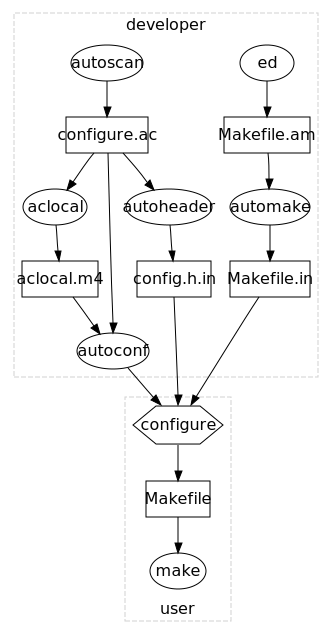
\includegraphics[width=7.5cm]{pictures/autoconf}
\end{center}
\label{fig:autoconf}
\caption{Etapes successives de la configuration d'un projet}
\end{figure}


\paragraph{}
Ce que l'on peut conclure de ce chapitre est que les outils de configuration des sources comme les
autotools sont tr�s puissants, mais complexes � comprendre du fait de leur richesse.\\
Cependant, du fait de leur usage tr�s fr�quent, ils restent incontournables d�s qu'il est
n�cessaire de consid�rer des projets au format sources, que ce soit pour cr�er un projet ou pour
construire un environnement embarqu�.

%%
%%
%% tests_profiling.tex for  in /doctorat/ece/partenariat/cours/outils_gnu
%%
%% Made by Philippe THIERRY
%% Login   <Philippe THIERRYreseau-libre.net>
%%
%% Started on  Wed Sep  1 18:08:07 2010 Philippe THIERRY
%% Last update Wed Sep 22 14:10:00 2010 Philippe THIERRY
%%

\chapter{Les outils de test et de profiling des applicatifs}


{\it Ce chapitre d�crit les diff�rents logiciels qui permettent de valider
le comportement de l'�l�ment produit. Il d�crit comment, dans le domaine
industriel, sont consid�r�s les outils et mesures de validation et de
profiling (�tude du profil d'ex�cution d'une tache, en terme d'appel de fonctions,
de consommation m�moire, etc).\\
Ces m�thodes de durcissement du logiciel sont tr�s importantes dans les
domaines de l'embarqu� critique, du temps r�el ou encore de la s�curit�
car ils sont � l'origine de la qualit� logicielle.}

\section{Du travail de d�veloppeur � l'ing�nieur en g�nie logiciel}

\paragraph{}
Au del� de la production logicielle telle que vue dans les paragraphes
pr�c�dents, il  convient de mettre en  {\oe}uvre d'autres  outils afin de
s'assurer de la bonne qualit� des logiciels.

\paragraph{}
Le  concept  de qualit� logicielle doit   �tre instanci� sur plusieurs
axes    au prorata des  objectifs  �  atteindre.  Parmi les diff�rents
crit�res que l'on   peut retenir, on peur citer :

\begin{itemize}
\item {\bf le taux  de commentaire}\\
C'est un point important, car  au del�  du langage utilis�, le logiciel
produit doit �tre comment� afin d'expliquer   soit des formules,
soit des constructions logicielles particuli�res.   Il faut consid�rer
�  ce  niveau qu'un logiciel doit  pouvoir �tre am�lior�, maintenu  et
corrig� par  des individus qui   n'ont    pas n�cessairement les m�mes
niveaux d'expertise  que  le ou les auteur(s)  original(aux). Ils n'ont
pas non   plus forc�ment la m�me approche de la conception du
logiciel.\\
Une  mani�re simple de mesurer les  commentaires consiste � �valuer  le
rapport  entre le  nombre de lignes  de code  et le nombre  de  lignes de
commentaires.  Une valeure correcte de  30\% est acceptable,   sous r�serve
que les  commentaires soient pertinents, ce qui h�las n'est pas ais� �
mesurer de mani�re automatique.

\item {\bf la capacit� � fournir  des  tests}\\
Dans la mesure   o� il  existe  un logiciel  r�alisant  une  fonction
particuli�re,  on peut s'attendre �  disposer de logiciels de test
permettant d'en assurer de mani�re plus  ou moins automatique la v�rification.\\
Un int�r�t  majeur des tests est la  capacit� � effectuer de  mani�re
automatique une v�rification de conformit� � des r�sultats attendus. Ils
fournissent de plus la possibilit� � terme d'effectuer  des tests de non
r�gression. Ces tests permettent, lors de l'ajout ou de la correction de
code, de s'assurer que le logiciel continue de r�ussir les tests pr�c�dement
valides. Dans le cas contraire, on parle de r�gression.\\
Il s'agit ici de la m�me id�e  que dans le domaine   automobile ou sur
les  chaines de production  de voitures : les robots  se calibrent seuls,
mesurent l'usure    de leurs outils et  v�rifient   pour  chaque pi�ce la bonne
conformit� sur  des �tats de surface par exemple.
Dans  le  monde  du logiciel, on parle alors de {\it tests unitaires}.\\
Ainsi, selon la d�coupe statique originale du projet  en fichiers sources,
on devrait trouver au moins un fichier de test par fichier source.  Chacun d'entre
eux doit g�n�rer un ex�cutable. Ce dernier a pour objectif d'appeler au moins une
fonction du logiciel �  tester, une ou plusieurs fois, afin de s'assurer que le r�sultat
produit par cette fonction est conforme � l'attendu. On parle alors de couverture
en {\it mode bloc}\\
Bien �videment,  de telles pratiques  sont tr�s co�teuse   dans  la
mesure ou    pour une  seule      ligne de code op�rationnelle, on  va
devoir r�diger environ trois � dix fois  plus de lignes de code de test,
dans le but de v�rifier divers cas d'usage de la fonction test�e.\\
Le nombre de lignes de code de test n�cessaires � valider le comportement d'une ligne de code
op�rationnelle n'est par fortuit. Il d�pend de la criticit� du logiciel.
Cela  d�pend du domaine d'activit� et  des enjeux du projet.
Par exemple, dans  le  cas de syst�mes critiques  (nucl�aire, militaire, avionique ou
satellite), il  est  demand� de faire des tests jusqu'� ce que {\it tous}
les  cas d'ex�cution de chaque ligne du logiciel   soient couverts.\\
Ceci  est   bien  d�fini dans une  norme internationale appell�e DO178B
dont l'objectif est de caract�riser de mani�re formelle  des syst�mes
complexes  � logiciels pr�pond�rants.\\
On peut donc conclure que selon le domaine dans lequel le logiciel est impl�ment�, l'effort de test
peut �tre soit peu couteux, soit beaucoup plus couteux que l'effort d'impl�mentation du logiciel
lui-m�me.
\end{itemize}

\section{Mesure du taux de counverture avec Gcov}

\paragraph{}
Il existe des outils pour mesurer le taux de couverture des ex�cutables de test d�crits au dessus.
Dans le monde open-source, il existe Gcov, qui fait parti de la suite gcc.\\
Il s'agit d'un outil de m�trologie du logiciel mode  bloc:\\
Lors de l'ex�cution des logiciels de test, cet outil permet, en concat�nant la couverture de chacun
d'entre eux, de d�finir, par bloc fonctionnel, quel sous ensemble du code du logiciel cible a �t�
test�.\\
Gcov ne n�cessite pas de construire un syst�me de tests automatiques, mais c'est cependant
fortement conseill�, car cela acc�l�re grandement la v�rification, au vue du nombre parfois grand
de logiciels de test. De plus, cela fournit un cadre formel � l'ex�cution des tests.\\
Le sch�ma \ref{fig:gcov} montre un exemple de r�sultat de taux de couverture sur du code C. Il
est indiqu� pour chaque ligne le nombre d'ex�cutions effectu�es. Les lignes n'ayant pas �t�
ex�cut�es sont indiqu�es en rouge.

\begin{figure}[ht]
\begin{center}
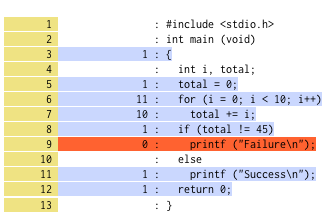
\includegraphics[width=6cm]{pictures/lcov}
\end{center}
\label{fig:gcov}
\caption{Taux de couverture par ligne de code avec Gcov}
\end{figure}



\paragraph{}
Sous r�serve de faire quelques efforts suppl�mentaires afin d'int�grer cet  outillage dans
le Makefile, on se  rapproche de  plus en  plus d'outillages industriels  comparables �
ceux de l'industrie automobile par exemple.\\
Les �l�ments que fournit gcov permettent de savoir si l'impl�mentation des campagnes de test sont
compatibles avec les exigences d'entr�e du logiciel. Ces derni�res sont souvent d�finies sous forme d'un
taux de couverture (en pourcentage). Le sch�ma pr�c�dent permet ainsi de savoir quand ce taux est
atteint. En effet, faire plus de tests que demand� implique un surco�t qu'il est pr�f�rable
d'�viter afin de respecter le devis initial.

\section{D�finition du profil d'ex�cution avec Gprof}

\paragraph{}
Au travers de l'ex�cution des logiciels de test il peut �tre  int�ressant
de v�rifier  le comportement temporel des fonctions test�es  en terme de boucles
et d'appel de  fonctions.  C'est le r�le de  l'outil {\texttt gprof}\index{Gprof}
qui �  l'instar de {\texttt gcov} va permettre de fournir des graphes permettant
d'analyser le bon comportement de ces derni�res. Il est de plus possible de mesurer le comportement
du logiciel lui m�me en simulant un environnement d'ex�cution repr�sentatif du besoin.\\
Le sch�ma \ref{fig:gprof} montre un arbre d'ex�cution d'un logiciel complet. Il indique l'arbre
d'appel des diff�rentes fonctions, ainsi que pour chacune, le nombre d'appels et le co�t relatif �
la dur�e d'ex�cution de chaque fonction. Cela permet entre autre de d�tecter les fonctions
anormalement longues.

\begin{figure}[ht]
\begin{center}
\begin{changemargin}{-1cm}{1cm}
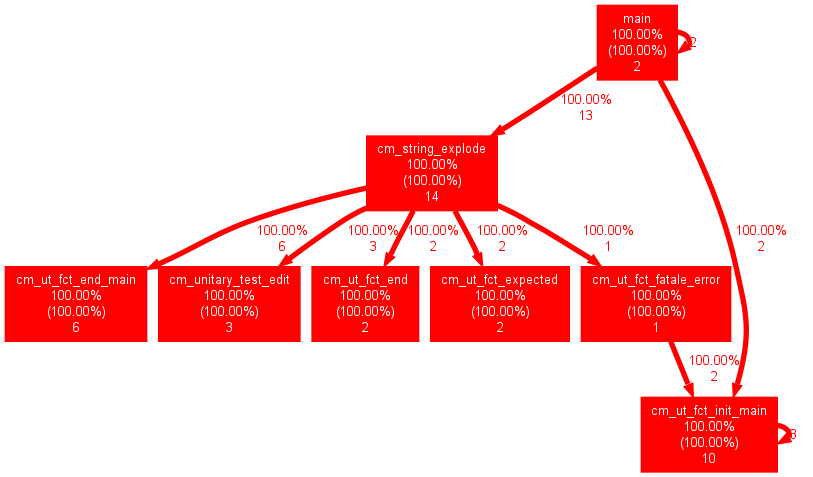
\includegraphics[width=18cm]{pictures/gprof_simple}
\end{changemargin}
\end{center}
\label{fig:gprof}
\caption{Exemple de graphe d'appel de fonctions r�sultant de l'ex�cution de GProf}
\end{figure}

\subsection{Mesurer la complexit� d'un source: pmccabe}

\paragraph{}
comme vu pr�c�demment,    compte  tenu    que   l'effort     de test    peut �tre
particuli�rement co�teux, il est int�ressant de savoir � l'avance quel
va �tre le co�t futur de la r�daction des  tests et par la m�me occasion le  co�t  de
maintenance  du  logiciel.   En  effet,  dans les grands  programmes
industriels o�   les dur�es  de  vie   des syst�mes   sont  importants
(nucl�aire,a�ronautique), est-il possible  d'�laborer un ou  plusieurs
crit�res  permettant de d�finir  le caract�re {\it complexe} du  logiciel ? 
Cette question est d'autant plus cruciale  que selon la r�ponse, l'effort de test peut �tre �tre
plus important et l'effort  de maintenance plus �lev�.

\paragraph{}
C'est � cette question que r�pond l'outil pmccabe, cr�� par George P. MacCabe, professeur
de statistique de l'universit� de Purdue University aux Etats Unis, dans le cadre de
sa th�se de statistiques appliqu�es � l'informatique.\\

\paragraph{}
Cet outil d�finit un indice de complexit� appartenant � l'ensemble des entiers positifs non nuls.
Cet  indice  s'appelle {\it complexit� cyclomatique}.  Il caract�rise, pour un bloc de code donn�,
la complexit� associ�e. Cela permet ainsi de d�finir une valeur cyclomatique pour une fonction, et
dans le cadre d'un projet complet une valeur cyclomatique moyenne.\\
Plus la valeur cyclomatique est �lev�e, plus la complexit� associ�e est grande. Des �l�ments
entrant en ligne de compte dans l'accroissement de la valeur cyclomatiques sont le nombre de branchements,
ou encore le nombre de sortie possible d'un bloc. En effet, plus leur nombre augmente, plus le
nombre de chemins d'ex�cution augmente, et plus le comportement du bloc devient complexe. Une
cons�quence directe est le nombre de fichiers de tests n�cessaire pour v�rifier les diff�rents
chemins d'ex�cution possible du bloc.\\
En �tudiant la plupart des logiciels open-source, on tombe r�guli�rement sur une valeur moyenne du
nombre cyclomatique d'environ 30, avec un certain nombre de fonctions pouvant atteindre 250 ou plus.
A titre   d'information,  on consid�re  qu'une   personne normale peut comprendre un logiciel
dont le nombre cyclomatique est inf�rieur � 9.\\
Dans certains projets industriels, l'exigence de valeur cyclomatique inf�rieure � 9 peut �tre
demand�e. Dans certains projets tr�s critiques, il peut �tre demand� une valeur cyclomatique ne
d�passant pas 6. Le meilleur moyen de ce rendre compte de ce que cela veut dire est de tester
l'outil sur quelques fonctions, afin de comprendre � quel point il peut �tre complexe de respecter
cette exigence.

\section{Validation de la configuration m�moire et de l'emploi des caches}

\subsection{Valgrind}

\paragraph{}
Valgrind est un outil open-source permettant de fournir des informations sur la consommation
m�moire dynamique d'un programme. Il ne n�cessite pas de recompiler le programme cible, son
fonctionnement s'appuyant sur une substitution des appels aux fonctions de gestion m�moire de la
libc par ces propres fonctions. Ceci permet, de mani�re transparente, de d�tecter des �l�ments
comme :
\begin{itemize}
\item La consommation m�moire lors d'une ex�cution donn�e
\item Le nombre d'allocations et de d�sallocations de m�moire
\item Les buffers overflows
\item Les fuites m�moire
\end{itemize}

\subsection{Cachegrind}

\paragraph{}
Cachegrind est un programme de la famille de Valgrind, mais qui se concentre sur la gestion du
cache de donn�es. Il prend un programme en argument et fournit, pour une ex�cution donn�e de
celui-ci, la consommation du cache de donn�e, le taux de cache-hits et de cache-miss, et d'autres
�l�ments d'information li�s aux caches.\\
Cachegrind impl�mente un simulateur d'algorithmes de caches de type LRU\footnote{{\it Least Recently
Used}, remplace la ligne de cache la moins souvent utilis�e} avec un cache � deux niveaux.
C'est d'ailleurs sa faiblesse : peu d'algorithmes de caches sont impl�ment�s. C'est cependant une
base tr�s int�ressante pour d�finir le profil de consommation de cache d'un programme.

\subsection{Mesurer la lourdeur d'un projet: sloccount}

\paragraph{}
Le programme {\it sloccount} est un binaire fournissant des donn�es de m�trologie sur les sources
d'un projet. Il fournit le nombre de lignes de code d�tect�es dans un fichier ou un r�pertoire, par
langage. Il fournit �galement le co�t th�orique de l'impl�mentation du projet, en heures et en
dollars, � partir du nombre de lignes de code trouv�es.

\section{Synth�se}

\paragraph{}
Il existe un grand nombre de projets fournissant des informations utiles tant au d�veloppeur qu'�
l'int�grateur. Ils sont peu employ�s par la communaut� mais ont une r�elle valeur ajout�e dans le
cadre de syst�mes industriels. Tous ces outils contribuent un m�tier : le g�nie logiciel.



\begin{appendices}
%%
%%
%% cpp_result.tex for  in /home/phil/Travail/ECE/cours/outils_gnu
%%
%% Made by Philippe THIERRY
%% Login   <Philippe THIERRYreseau-libre.net>
%%
%% Started on  mer. 01 sept. 2010 21:30:33 CEST Philippe THIERRY
%% Last update mer. 01 sept. 2010 21:32:29 CEST Philippe THIERRY
%%

\chapter{Sortie du traitement du pr�processeur}

Comme vu dans le Chapitre \ref{preproc}, le fichier r�sultant du traitement du pr�processing est volumineux. En voici le contenu :
\begin{lstlisting}
# 1 "example_cpp.c"
# 1 "<built-in>"
# 1 "<command-line>"
# 1 "example_cpp.c"
# 27 "example_cpp.c"
# 1 "/usr/include/stdio.h" 1 3 4
# 28 "/usr/include/stdio.h" 3 4
# 1 "/usr/include/features.h" 1 3 4
# 313 "/usr/include/features.h" 3 4
# 1 "/usr/include/bits/predefs.h" 1 3 4
# 314 "/usr/include/features.h" 2 3 4
# 346 "/usr/include/features.h" 3 4
# 1 "/usr/include/sys/cdefs.h" 1 3 4
# 353 "/usr/include/sys/cdefs.h" 3 4
# 1 "/usr/include/bits/wordsize.h" 1 3 4
# 354 "/usr/include/sys/cdefs.h" 2 3 4
# 347 "/usr/include/features.h" 2 3 4
# 378 "/usr/include/features.h" 3 4
# 1 "/usr/include/gnu/stubs.h" 1 3 4



# 1 "/usr/include/bits/wordsize.h" 1 3 4
# 5 "/usr/include/gnu/stubs.h" 2 3 4




# 1 "/usr/include/gnu/stubs-64.h" 1 3 4
# 10 "/usr/include/gnu/stubs.h" 2 3 4
# 379 "/usr/include/features.h" 2 3 4
# 29 "/usr/include/stdio.h" 2 3 4





# 1 "/usr/lib/gcc/x86_64-linux-gnu/4.4.3/include/stddef.h" 1 3 4
# 211 "/usr/lib/gcc/x86_64-linux-gnu/4.4.3/include/stddef.h" 3 4
typedef long unsigned int size_t;
# 35 "/usr/include/stdio.h" 2 3 4

# 1 "/usr/include/bits/types.h" 1 3 4
# 28 "/usr/include/bits/types.h" 3 4
# 1 "/usr/include/bits/wordsize.h" 1 3 4
# 29 "/usr/include/bits/types.h" 2 3 4


typedef unsigned char __u_char;
typedef unsigned short int __u_short;
typedef unsigned int __u_int;
typedef unsigned long int __u_long;


typedef signed char __int8_t;
typedef unsigned char __uint8_t;
typedef signed short int __int16_t;
typedef unsigned short int __uint16_t;
typedef signed int __int32_t;
typedef unsigned int __uint32_t;

typedef signed long int __int64_t;
typedef unsigned long int __uint64_t;







typedef long int __quad_t;
typedef unsigned long int __u_quad_t;
# 131 "/usr/include/bits/types.h" 3 4
# 1 "/usr/include/bits/typesizes.h" 1 3 4
# 132 "/usr/include/bits/types.h" 2 3 4


typedef unsigned long int __dev_t;
typedef unsigned int __uid_t;
typedef unsigned int __gid_t;
typedef unsigned long int __ino_t;
typedef unsigned long int __ino64_t;
typedef unsigned int __mode_t;
typedef unsigned long int __nlink_t;
typedef long int __off_t;
typedef long int __off64_t;
typedef int __pid_t;
typedef struct { int __val[2]; } __fsid_t;
typedef long int __clock_t;
typedef unsigned long int __rlim_t;
typedef unsigned long int __rlim64_t;
typedef unsigned int __id_t;
typedef long int __time_t;
typedef unsigned int __useconds_t;
typedef long int __suseconds_t;

typedef int __daddr_t;
typedef long int __swblk_t;
typedef int __key_t;


typedef int __clockid_t;


typedef void * __timer_t;


typedef long int __blksize_t;




typedef long int __blkcnt_t;
typedef long int __blkcnt64_t;


typedef unsigned long int __fsblkcnt_t;
typedef unsigned long int __fsblkcnt64_t;


typedef unsigned long int __fsfilcnt_t;
typedef unsigned long int __fsfilcnt64_t;

typedef long int __ssize_t;



typedef __off64_t __loff_t;
typedef __quad_t *__qaddr_t;
typedef char *__caddr_t;


typedef long int __intptr_t;


typedef unsigned int __socklen_t;
# 37 "/usr/include/stdio.h" 2 3 4
# 45 "/usr/include/stdio.h" 3 4
struct _IO_FILE;



typedef struct _IO_FILE FILE;





# 65 "/usr/include/stdio.h" 3 4
typedef struct _IO_FILE __FILE;
# 75 "/usr/include/stdio.h" 3 4
# 1 "/usr/include/libio.h" 1 3 4
# 32 "/usr/include/libio.h" 3 4
# 1 "/usr/include/_G_config.h" 1 3 4
# 15 "/usr/include/_G_config.h" 3 4
# 1 "/usr/lib/gcc/x86_64-linux-gnu/4.4.3/include/stddef.h" 1 3 4
# 16 "/usr/include/_G_config.h" 2 3 4




# 1 "/usr/include/wchar.h" 1 3 4
# 83 "/usr/include/wchar.h" 3 4
typedef struct
{
  int __count;
  union
  {

    unsigned int __wch;



    char __wchb[4];
  } __value;
} __mbstate_t;
# 21 "/usr/include/_G_config.h" 2 3 4

typedef struct
{
  __off_t __pos;
  __mbstate_t __state;
} _G_fpos_t;
typedef struct
{
  __off64_t __pos;
  __mbstate_t __state;
} _G_fpos64_t;
# 53 "/usr/include/_G_config.h" 3 4
typedef int _G_int16_t __attribute__ ((__mode__ (__HI__)));
typedef int _G_int32_t __attribute__ ((__mode__ (__SI__)));
typedef unsigned int _G_uint16_t __attribute__ ((__mode__ (__HI__)));
typedef unsigned int _G_uint32_t __attribute__ ((__mode__ (__SI__)));
# 33 "/usr/include/libio.h" 2 3 4
# 53 "/usr/include/libio.h" 3 4
# 1 "/usr/lib/gcc/x86_64-linux-gnu/4.4.3/include/stdarg.h" 1 3 4
# 40 "/usr/lib/gcc/x86_64-linux-gnu/4.4.3/include/stdarg.h" 3 4
typedef __builtin_va_list __gnuc_va_list;
# 54 "/usr/include/libio.h" 2 3 4
# 170 "/usr/include/libio.h" 3 4
struct _IO_jump_t; struct _IO_FILE;
# 180 "/usr/include/libio.h" 3 4
typedef void _IO_lock_t;





struct _IO_marker {
  struct _IO_marker *_next;
  struct _IO_FILE *_sbuf;



  int _pos;
# 203 "/usr/include/libio.h" 3 4
};


enum __codecvt_result
{
  __codecvt_ok,
  __codecvt_partial,
  __codecvt_error,
  __codecvt_noconv
};
# 271 "/usr/include/libio.h" 3 4
struct _IO_FILE {
  int _flags;




  char* _IO_read_ptr;
  char* _IO_read_end;
  char* _IO_read_base;
  char* _IO_write_base;
  char* _IO_write_ptr;
  char* _IO_write_end;
  char* _IO_buf_base;
  char* _IO_buf_end;

  char *_IO_save_base;
  char *_IO_backup_base;
  char *_IO_save_end;

  struct _IO_marker *_markers;

  struct _IO_FILE *_chain;

  int _fileno;



  int _flags2;

  __off_t _old_offset;



  unsigned short _cur_column;
  signed char _vtable_offset;
  char _shortbuf[1];



  _IO_lock_t *_lock;
# 319 "/usr/include/libio.h" 3 4
  __off64_t _offset;
# 328 "/usr/include/libio.h" 3 4
  void *__pad1;
  void *__pad2;
  void *__pad3;
  void *__pad4;
  size_t __pad5;

  int _mode;

  char _unused2[15 * sizeof (int) - 4 * sizeof (void *) - sizeof (size_t)];

};


typedef struct _IO_FILE _IO_FILE;


struct _IO_FILE_plus;

extern struct _IO_FILE_plus _IO_2_1_stdin_;
extern struct _IO_FILE_plus _IO_2_1_stdout_;
extern struct _IO_FILE_plus _IO_2_1_stderr_;
# 364 "/usr/include/libio.h" 3 4
typedef __ssize_t __io_read_fn (void *__cookie, char *__buf, size_t __nbytes);







typedef __ssize_t __io_write_fn (void *__cookie, __const char *__buf,
     size_t __n);







typedef int __io_seek_fn (void *__cookie, __off64_t *__pos, int __w);


typedef int __io_close_fn (void *__cookie);
# 416 "/usr/include/libio.h" 3 4
extern int __underflow (_IO_FILE *);
extern int __uflow (_IO_FILE *);
extern int __overflow (_IO_FILE *, int);
# 460 "/usr/include/libio.h" 3 4
extern int _IO_getc (_IO_FILE *__fp);
extern int _IO_putc (int __c, _IO_FILE *__fp);
extern int _IO_feof (_IO_FILE *__fp) __attribute__ ((__nothrow__));
extern int _IO_ferror (_IO_FILE *__fp) __attribute__ ((__nothrow__));

extern int _IO_peekc_locked (_IO_FILE *__fp);





extern void _IO_flockfile (_IO_FILE *) __attribute__ ((__nothrow__));
extern void _IO_funlockfile (_IO_FILE *) __attribute__ ((__nothrow__));
extern int _IO_ftrylockfile (_IO_FILE *) __attribute__ ((__nothrow__));
# 490 "/usr/include/libio.h" 3 4
extern int _IO_vfscanf (_IO_FILE * __restrict, const char * __restrict,
   __gnuc_va_list, int *__restrict);
extern int _IO_vfprintf (_IO_FILE *__restrict, const char *__restrict,
    __gnuc_va_list);
extern __ssize_t _IO_padn (_IO_FILE *, int, __ssize_t);
extern size_t _IO_sgetn (_IO_FILE *, void *, size_t);

extern __off64_t _IO_seekoff (_IO_FILE *, __off64_t, int, int);
extern __off64_t _IO_seekpos (_IO_FILE *, __off64_t, int);

extern void _IO_free_backup_area (_IO_FILE *) __attribute__ ((__nothrow__));
# 76 "/usr/include/stdio.h" 2 3 4
# 89 "/usr/include/stdio.h" 3 4


typedef _G_fpos_t fpos_t;




# 141 "/usr/include/stdio.h" 3 4
# 1 "/usr/include/bits/stdio_lim.h" 1 3 4
# 142 "/usr/include/stdio.h" 2 3 4



extern struct _IO_FILE *stdin;
extern struct _IO_FILE *stdout;
extern struct _IO_FILE *stderr;







extern int remove (__const char *__filename) __attribute__ ((__nothrow__));

extern int rename (__const char *__old, __const char *__new) __attribute__ ((__nothrow__));




extern int renameat (int __oldfd, __const char *__old, int __newfd,
       __const char *__new) __attribute__ ((__nothrow__));








extern FILE *tmpfile (void) ;
# 186 "/usr/include/stdio.h" 3 4
extern char *tmpnam (char *__s) __attribute__ ((__nothrow__)) ;





extern char *tmpnam_r (char *__s) __attribute__ ((__nothrow__)) ;
# 204 "/usr/include/stdio.h" 3 4
extern char *tempnam (__const char *__dir, __const char *__pfx)
     __attribute__ ((__nothrow__)) __attribute__ ((__malloc__)) ;








extern int fclose (FILE *__stream);




extern int fflush (FILE *__stream);

# 229 "/usr/include/stdio.h" 3 4
extern int fflush_unlocked (FILE *__stream);
# 243 "/usr/include/stdio.h" 3 4






extern FILE *fopen (__const char *__restrict __filename,
      __const char *__restrict __modes) ;




extern FILE *freopen (__const char *__restrict __filename,
        __const char *__restrict __modes,
        FILE *__restrict __stream) ;
# 272 "/usr/include/stdio.h" 3 4

# 283 "/usr/include/stdio.h" 3 4
extern FILE *fdopen (int __fd, __const char *__modes) __attribute__ ((__nothrow__)) ;
# 296 "/usr/include/stdio.h" 3 4
extern FILE *fmemopen (void *__s, size_t __len, __const char *__modes)
  __attribute__ ((__nothrow__)) ;




extern FILE *open_memstream (char **__bufloc, size_t *__sizeloc) __attribute__ ((__nothrow__)) ;






extern void setbuf (FILE *__restrict __stream, char *__restrict __buf) __attribute__ ((__nothrow__));



extern int setvbuf (FILE *__restrict __stream, char *__restrict __buf,
      int __modes, size_t __n) __attribute__ ((__nothrow__));





extern void setbuffer (FILE *__restrict __stream, char *__restrict __buf,
         size_t __size) __attribute__ ((__nothrow__));


extern void setlinebuf (FILE *__stream) __attribute__ ((__nothrow__));








extern int fprintf (FILE *__restrict __stream,
      __const char *__restrict __format, ...);




extern int printf (__const char *__restrict __format, ...);

extern int sprintf (char *__restrict __s,
      __const char *__restrict __format, ...) __attribute__ ((__nothrow__));





extern int vfprintf (FILE *__restrict __s, __const char *__restrict __format,
       __gnuc_va_list __arg);




extern int vprintf (__const char *__restrict __format, __gnuc_va_list __arg);

extern int vsprintf (char *__restrict __s, __const char *__restrict __format,
       __gnuc_va_list __arg) __attribute__ ((__nothrow__));





extern int snprintf (char *__restrict __s, size_t __maxlen,
       __const char *__restrict __format, ...)
     __attribute__ ((__nothrow__)) __attribute__ ((__format__ (__printf__, 3, 4)));

extern int vsnprintf (char *__restrict __s, size_t __maxlen,
        __const char *__restrict __format, __gnuc_va_list __arg)
     __attribute__ ((__nothrow__)) __attribute__ ((__format__ (__printf__, 3, 0)));

# 394 "/usr/include/stdio.h" 3 4
extern int vdprintf (int __fd, __const char *__restrict __fmt,
       __gnuc_va_list __arg)
     __attribute__ ((__format__ (__printf__, 2, 0)));
extern int dprintf (int __fd, __const char *__restrict __fmt, ...)
     __attribute__ ((__format__ (__printf__, 2, 3)));








extern int fscanf (FILE *__restrict __stream,
     __const char *__restrict __format, ...) ;




extern int scanf (__const char *__restrict __format, ...) ;

extern int sscanf (__const char *__restrict __s,
     __const char *__restrict __format, ...) __attribute__ ((__nothrow__));
# 425 "/usr/include/stdio.h" 3 4
extern int fscanf (FILE *__restrict __stream, __const char *__restrict __format, ...) __asm__ ("" "__isoc99_fscanf") ;


extern int scanf (__const char *__restrict __format, ...) __asm__ ("" "__isoc99_scanf") ;

extern int sscanf (__const char *__restrict __s, __const char *__restrict __format, ...) __asm__ ("" "__isoc99_sscanf") __attribute__ ((__nothrow__));
# 445 "/usr/include/stdio.h" 3 4








extern int vfscanf (FILE *__restrict __s, __const char *__restrict __format,
      __gnuc_va_list __arg)
     __attribute__ ((__format__ (__scanf__, 2, 0))) ;





extern int vscanf (__const char *__restrict __format, __gnuc_va_list __arg)
     __attribute__ ((__format__ (__scanf__, 1, 0))) ;


extern int vsscanf (__const char *__restrict __s,
      __const char *__restrict __format, __gnuc_va_list __arg)
     __attribute__ ((__nothrow__)) __attribute__ ((__format__ (__scanf__, 2, 0)));
# 476 "/usr/include/stdio.h" 3 4
extern int vfscanf (FILE *__restrict __s, __const char *__restrict __format, __gnuc_va_list __arg) __asm__ ("" "__isoc99_vfscanf")



     __attribute__ ((__format__ (__scanf__, 2, 0))) ;
extern int vscanf (__const char *__restrict __format, __gnuc_va_list __arg) __asm__ ("" "__isoc99_vscanf")

     __attribute__ ((__format__ (__scanf__, 1, 0))) ;
extern int vsscanf (__const char *__restrict __s, __const char *__restrict __format, __gnuc_va_list __arg) __asm__ ("" "__isoc99_vsscanf")



     __attribute__ ((__nothrow__)) __attribute__ ((__format__ (__scanf__, 2, 0)));
# 504 "/usr/include/stdio.h" 3 4









extern int fgetc (FILE *__stream);
extern int getc (FILE *__stream);





extern int getchar (void);

# 532 "/usr/include/stdio.h" 3 4
extern int getc_unlocked (FILE *__stream);
extern int getchar_unlocked (void);
# 543 "/usr/include/stdio.h" 3 4
extern int fgetc_unlocked (FILE *__stream);











extern int fputc (int __c, FILE *__stream);
extern int putc (int __c, FILE *__stream);





extern int putchar (int __c);

# 576 "/usr/include/stdio.h" 3 4
extern int fputc_unlocked (int __c, FILE *__stream);







extern int putc_unlocked (int __c, FILE *__stream);
extern int putchar_unlocked (int __c);






extern int getw (FILE *__stream);


extern int putw (int __w, FILE *__stream);








extern char *fgets (char *__restrict __s, int __n, FILE *__restrict __stream)
     ;






extern char *gets (char *__s) ;

# 638 "/usr/include/stdio.h" 3 4
extern __ssize_t __getdelim (char **__restrict __lineptr,
          size_t *__restrict __n, int __delimiter,
          FILE *__restrict __stream) ;
extern __ssize_t getdelim (char **__restrict __lineptr,
        size_t *__restrict __n, int __delimiter,
        FILE *__restrict __stream) ;







extern __ssize_t getline (char **__restrict __lineptr,
       size_t *__restrict __n,
       FILE *__restrict __stream) ;








extern int fputs (__const char *__restrict __s, FILE *__restrict __stream);





extern int puts (__const char *__s);






extern int ungetc (int __c, FILE *__stream);






extern size_t fread (void *__restrict __ptr, size_t __size,
       size_t __n, FILE *__restrict __stream) ;




extern size_t fwrite (__const void *__restrict __ptr, size_t __size,
        size_t __n, FILE *__restrict __s);

# 710 "/usr/include/stdio.h" 3 4
extern size_t fread_unlocked (void *__restrict __ptr, size_t __size,
         size_t __n, FILE *__restrict __stream) ;
extern size_t fwrite_unlocked (__const void *__restrict __ptr, size_t __size,
          size_t __n, FILE *__restrict __stream);








extern int fseek (FILE *__stream, long int __off, int __whence);




extern long int ftell (FILE *__stream) ;




extern void rewind (FILE *__stream);

# 746 "/usr/include/stdio.h" 3 4
extern int fseeko (FILE *__stream, __off_t __off, int __whence);




extern __off_t ftello (FILE *__stream) ;
# 765 "/usr/include/stdio.h" 3 4






extern int fgetpos (FILE *__restrict __stream, fpos_t *__restrict __pos);




extern int fsetpos (FILE *__stream, __const fpos_t *__pos);
# 788 "/usr/include/stdio.h" 3 4

# 797 "/usr/include/stdio.h" 3 4


extern void clearerr (FILE *__stream) __attribute__ ((__nothrow__));

extern int feof (FILE *__stream) __attribute__ ((__nothrow__)) ;

extern int ferror (FILE *__stream) __attribute__ ((__nothrow__)) ;




extern void clearerr_unlocked (FILE *__stream) __attribute__ ((__nothrow__));
extern int feof_unlocked (FILE *__stream) __attribute__ ((__nothrow__)) ;
extern int ferror_unlocked (FILE *__stream) __attribute__ ((__nothrow__)) ;








extern void perror (__const char *__s);






# 1 "/usr/include/bits/sys_errlist.h" 1 3 4
# 27 "/usr/include/bits/sys_errlist.h" 3 4
extern int sys_nerr;
extern __const char *__const sys_errlist[];
# 827 "/usr/include/stdio.h" 2 3 4




extern int fileno (FILE *__stream) __attribute__ ((__nothrow__)) ;




extern int fileno_unlocked (FILE *__stream) __attribute__ ((__nothrow__)) ;
# 846 "/usr/include/stdio.h" 3 4
extern FILE *popen (__const char *__command, __const char *__modes) ;





extern int pclose (FILE *__stream);





extern char *ctermid (char *__s) __attribute__ ((__nothrow__));
# 886 "/usr/include/stdio.h" 3 4
extern void flockfile (FILE *__stream) __attribute__ ((__nothrow__));



extern int ftrylockfile (FILE *__stream) __attribute__ ((__nothrow__)) ;


extern void funlockfile (FILE *__stream) __attribute__ ((__nothrow__));
# 916 "/usr/include/stdio.h" 3 4

# 28 "example_cpp.c" 2



int foo(char *bar);

int foo(char *bar)
{
  bar += 12;
  return 0;
}
\end{lstlisting}

\end{appendices}

\backmatter

%\printglossary

% bibliography
%\nocite{*}
%\bibliography{bibliography}
%\bibliographystyle{plain}

\printindex

\end{document}
